\documentclass[times, utf8, zavrsni]{fer}
\usepackage{booktabs}
\usepackage{indentfirst}
\usepackage{amsmath}

\usepackage{minted}
%\BeforeBeginEnvironment{minted}{\medskip}
\AfterEndEnvironment{minted}{\medskip}


\usepackage{caption}
\usepackage[hidelinks]{hyperref}

\usepackage{xurl}
%\usepackage{breakurl}
%\usepackage{url}

%\usepackage{amssymb}
\usemintedstyle{vs}

\begin{document}
\urlstyle{rm}
% TODO: Navedite broj rada.
\thesisnumber{000}

% TODO: Navedite naslov rada.
\title{Mobilna aplikacija za klasifikaciju kožnih oboljenja iz slika kože}

% TODO: Navedite vaše ime i prezime.
\author{Petar Miličević}

\maketitle

% Ispis stranice s napomenom o umetanju izvornika rada. Uklonite naredbu \izvornik ako želite izbaciti tu stranicu.
\izvornik{}

% Dodavanje zahvale ili prazne stranice. Ako ne želite dodati zahvalu, naredbu ostavite radi prazne stranice.
\zahvala{}

\tableofcontents

\chapter{Uvod}

\indent{}
Strojno učenje jedna je od najbrže rastućih grana umjetne inteligencije. Glavni aspekt strojnog učenja koji ga odvaja od ostalih tehnika u umjetnoj inteligenciji je sposobnost prilagodbe i automatskog poboljšavanja algoritama kada su izloženi novim skupovima podataka. Zbog toga se smatra vrlo dinamičnim područjem koje ne ovisi toliko o ljudskim resursima kako bi se došlo do poboljšanja i novih saznanja [11].\\
%
\indent{}
Algoritmi strojnog učenja grade model zasnovan na ulaznom skupu podataka \engl{training data}. Pomoću izgrađenog modela algoritmi potom mogu donositi samostalne odluke i predviđanja bez da su za to eksplicitno programirani. U zadnjem desetljeću algoritmi strojnog učenja omogućili su razvoj autonomne vožnje, učinkovitije pretraživanje sadržaja na webu i automatsko prepoznavanje ljudskog govora, kao i mnogih drugih područja i primjena [12].\\
%
\indent{}
Duboko učenje jedna je od tehnika strojnog učenja. Algoritmi dubokog učenja zasnivaju se na modelima dubokih neuronskih mreža. Duboke neuronske mreže su skup algoritama koji postižu najveće postotke točnosti za razne važne probleme, kao što su prepoznavanje slika i zvuka. Termin "duboke" odnosi se na broj slojeva u neuronskoj mreži, tako postoje mreže s jednim i više tzv. "skrivenih slojeva" \engl{hidden layer}. Više takvih skrivenih slojeva omogućava dubokim neuronskim mrežama da na temeljitiji način nauče podatkovne značajke i njihovu hijerarhiju. Neke jednostavnije značajke rekombiniraju se iz jednog sloja u sljedeći pa je omogućeno stvaranje složenijih značajki, što rezultira dubljim poznavanjem podatkovnih međuovisnosti i obrazaca. Mreže s mnogo slojeva provode ulazni skup podataka kroz više skrivenih slojeva pa su stoga nerijetko vremenski zahtjevne za treniranje [11].\\
\newpage
%
\begin{figure}[!h]
\hspace{0.1\textwidth}
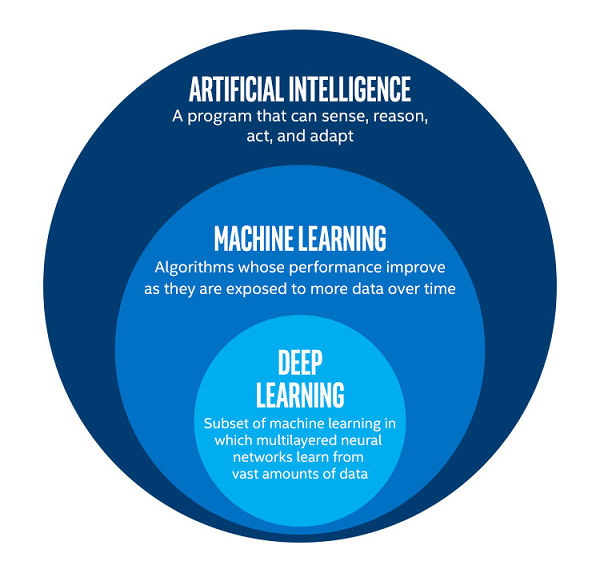
\includegraphics[width=0.8\textwidth]{./slike/AI-Circle.png}
\caption{Hijerarija područja umjetne inteligencije [1]}
\label{fig:ai-područja}
\end{figure}
%
\indent{}
Navedena područja imaju poseban značaj u razvoju medicine. Zahvaljujući postupcima strojnog učenja, liječnici mogu davati preciznije dijagnoze pacijentima, prognozirati daljnji razvoj nekih bolesti i predlagati prilagođenije načine liječenja [13]. Ovaj rad razmatra razvoj cjelokupnog rješenja, mobilne aplikacije koja omogućava klasifikaciju kožnih oboljenja na temelju slika kože.


\chapter{Koža i kožne bolesti}

\indent{}
Koža je najveći i najteži ljudski organ jer ima površinu od $1.2$ do $2.3$ $m^2$, a masa joj čini od 10 do 15 posto ukupne tjelesne mase [14].\\
%
\indent{}
S druge strane, rak kože najčešći je zloćudni tumor kod čovjeka. Povećanjem brzine rasta svoje incidencije u općoj populaciji, zadnja tri desetljeća izuzetno je izražen javnozdravstveni problem s kojim se bave gotovo sve zemlje u svijetu, pa tako i Republika Hrvatska. Prema posljednjim dostupnim informacijama Registra za rak Hrvatskog zavoda za javno zdravstvo, u 2014. godini bilo je ukupno 587 novooboljelih od melanoma, od toga 305 muškaraca i 282 žene. U dobnoj skupini od  30 do 39 godina jedan je od tri najčešća zloćudna tumora, uz karcinom testisa i štitnjače [14].\\
%
\indent{}
U većini slučajeva dijagnosticira se vizualno, počevši s početnim dermatološkim pregledom. Takav pristup otvara mogućnost uporabe algoritama dubokog učenja za pomoć u klasifikaciji oboljenja. Automatska klasifikacija kožnih oboljenja korištenjem slika izazovan je zadatak zbog velike varijabilnosti i nepravilnosti njihova izgleda.


\section{Koža}

\indent{}
Kao što je već spomenuto, koža je najveći ljudski organ. S kosom, noktima, žlijezdama i živcima dio je čovjekovog zaštitnog sustava koji djeluje kao prepreka između vanjske i unutarnje strane tijela. Debljina kože razlikuje se ovisno o dijelu tijela, najdeblja je na tabanima, oko $4$ $mm$, a najtanja na vjeđama, oko $0.2$ $mm$ [14].\\
%
\indent{}
Koža se sastoji od tri sloja tkiva: epidermisa, dermisa i hipodermisa.
\newpage{}
%
\textbf{Epidermis}\\
\indent{}
Epidermis je vanjski, vidljivi dio kože. Stanice epidermisa svakodnevno se obnavljaju jer se mrtve stanice neprestano odvajaju od ostatka tkiva. Glavne funkcije epidermisa su:
\begin{itemize}
\item[$\bullet$] Izrada novih kožnih stanica
\item[$\bullet$] Davanje boje koži
\item[$\bullet$] Zaštita kože
\end{itemize}

\textbf{Dermis}\\
\indent{}
Dermis je srednji sloj kože koji se nalazi ispod epidermisa. To je najdeblji sloj kože koji sadrži živce i krvne žile. U njemu se također nalaze znojne i uljne žlijezde, kao i korijeni dlaka. Sastoji se uglavnom od proteina kolagena koji kožu čini rastezljivom i snažnom. Glavne funkcije dermisa su:
\begin{itemize}
\item[$\bullet$] Osjet boli i dodira
\item[$\bullet$] Proizvodnja ulja i znoja
\item[$\bullet$] Rast dlaka i kose
\item[$\bullet$] Kontrola temperature kože
\item[$\bullet$] Borba protiv infekcije
\end{itemize}

\textbf{Hipodermis}\\
\indent{}
Hipodermis je najdublji sloj kože, najčešće se koristi kao sinonim za potkožno masno tkivo. Glavne funkcije hipodermisa su:
\begin{itemize}
\item[$\bullet$] Izolacija tijela od topline i hladnoće
\item[$\bullet$] Skladište energije
\item[$\bullet$] Zaštita unutarnjih organa i kostiju [14]
\end{itemize}
%
\begin{figure}[!h]
%\centering
%\vspace{-0.05\textwidth}
\hspace{0.3\textwidth}
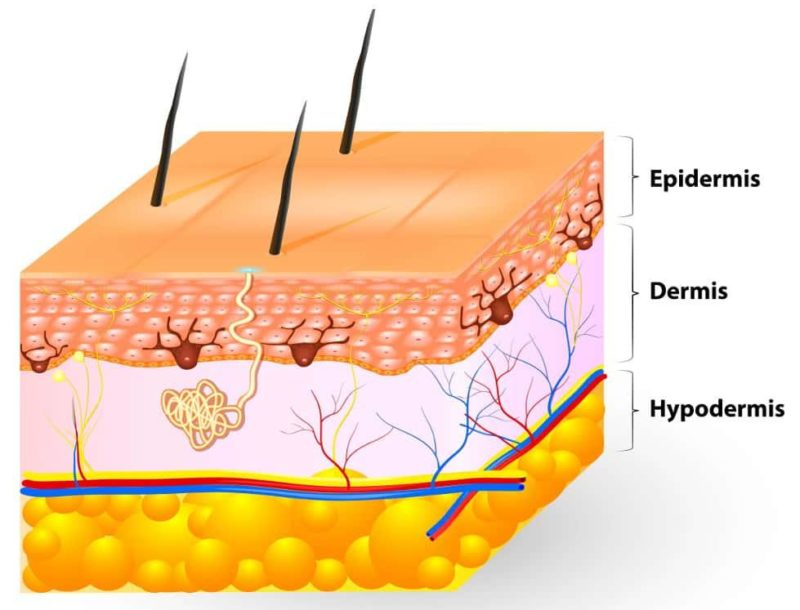
\includegraphics[width=0.4\textwidth]{./slike/skin2}
\caption{Slojevi kože [2]}
\label{fig:koza-slojevi}
\end{figure}
%


\section{Kožne bolesti}

Rak kože glavni je javnozdravstveni problem u svijetu, s više od $123000$ novih slučajeva svake godine. Najčešći je oblik karcinoma, koji čini oko $40$ posto ukupnog broja slučajeva raka [14]. Iako općenito postoji velik broj kožnih bolesti, u ovom radu fokus će biti na najčešće, tj. one koje su prisutne u skupu podataka koji će biti korišten za učenje i optimizaciju modela duboke neuronske mreže za klasifikaciju. Takav konkretan skup podataka-$HAM10000$ $dataset$ [15]. Skup podataka $HAM10000$ sastoji se od $10015$ slika kožnih oboljenja koje su objavljene kao skup ulaznih podataka za potrebe razvoja akademskog strojnog učenja. Skup podataka sadrži $7$ različitih klasa kožnih oboljenja koja su navedena u nastavku:

\begin{enumerate}
\item Melanocytic nevi -- Melanocitni nevusi(madeži) su dobroćudne(benigne) pigmentirane promjene građene od nevusnih stanica, melanocita. Obično se pojavljuju na koži i sluznicama, a prosječan broj melanocitnih nevusa kod odrasle osobe je od $20$ do $40$.

\item Melanoma -- Melanom je zloćudni tumor koji nastaje iz melanocita-specijaliziranih stanica koje proizvode melanin, a nalaze se u dubokom sloju epidermisa. Melanin je prirodni kožni pigment koji daje boju koži, kosi i očima. Ako se otkrije u ranoj fazi, može se izliječiti jednostavnim kirurškim zahvatom, melanomi također mogu biti invazivni i neinvazivni(in situ). 

\item Benign keratosis-like lesions -- Benigna(seboroična) keratoza jedna je od najčešćih nekanceroznih izraslina na koži u starijih osoba. Obično se pojavljuje kao smeđa ili crna izraslina na licu, prsima, ramenima ili leđima. Često se pojavljuje u skupinama, a općenito je bezbolna i ne zahtijeva liječenje.

\item Basal cell carcinoma -- Karcinom bazalnih stanica najčešća je vrsta kožnog karcinoma. Tumori započinju kao male čvrste uzdignute izrasline na koži ili rane nalik krastama. Rijetko stvara metastaze, ali destruktivno raste ako se ne liječi.

\item Actinic keratoses -- Aktinična keratoza očituje se kao keratonična tvorba na dijelovima kože koji su izloženi ultraljubičastom(UV) zračenju sunca. Može prijeći u zloćudni(maligni) planocelularni karcinom(rak pločastih stanica). Jedna je od najčešćih kožnih bolesti.

\item Vascular lesions -- Vaskularne lezije obuhvaćaju većinski bezopasne kožne izrasline. Ovdje spadaju angiom trešnje \engl{cherry angiomas}, anigokeratom \engl{anigokeratomas} i pilogeni granulom \engl{pyogenic granulomas}.

\item Dermatofibroma -- Fibrom ili dermatofibrom je benigna kožna izraslina građena od vlaknastog i vezivnog tkiva. Uglavnom je boje kože, no može biti i pigmentiran. Ne zahtijeva liječenje [14].

\end{enumerate}
%
\begin{figure}[!h]
\hspace{-0.05\textwidth}
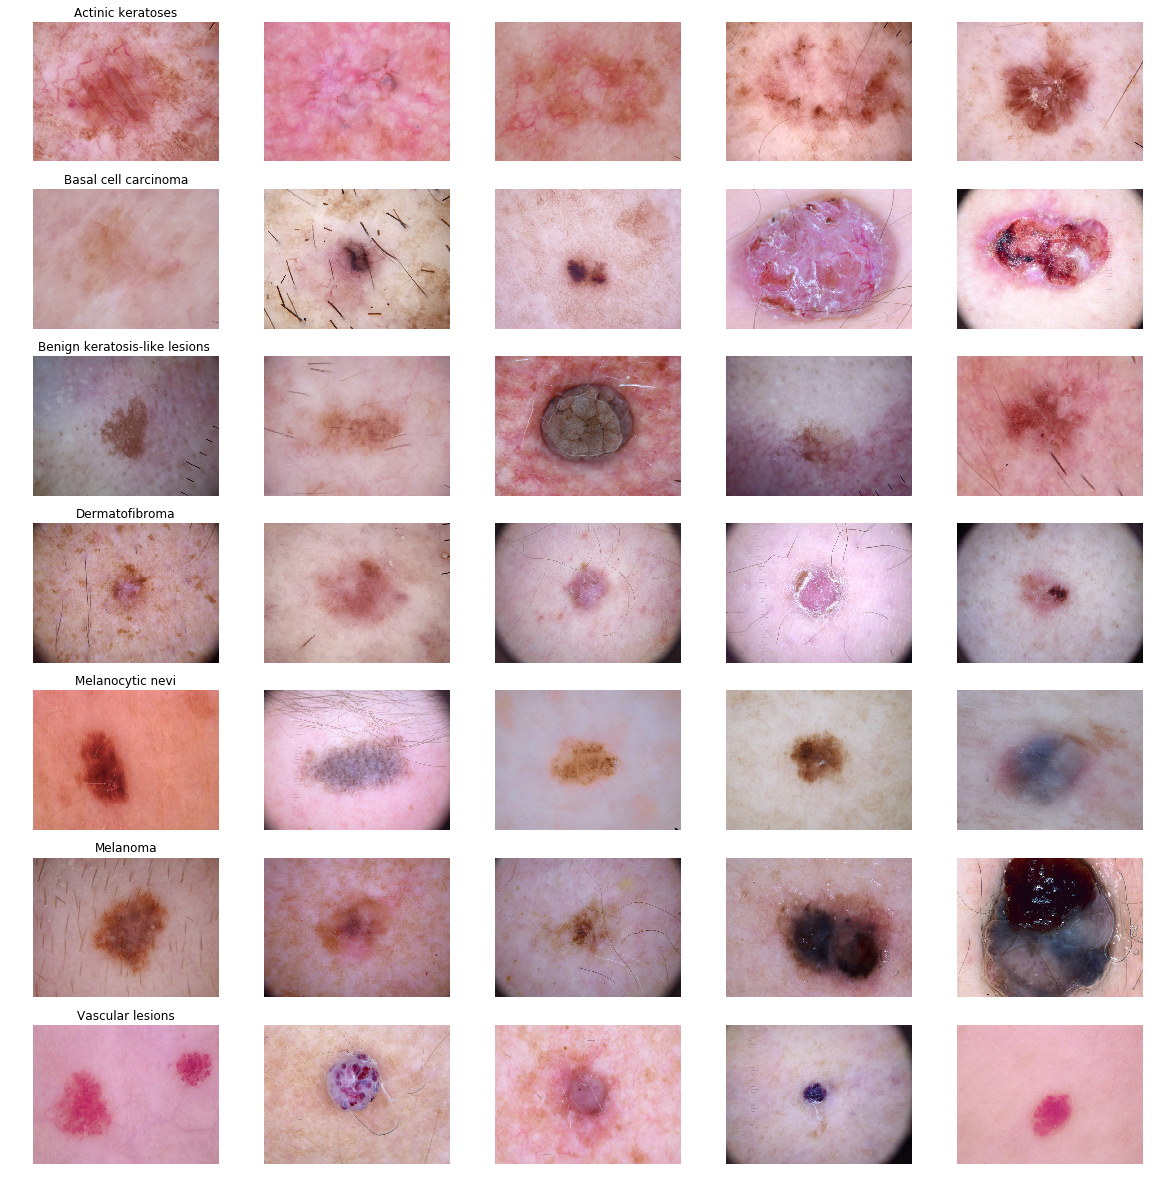
\includegraphics[width=1.1\textwidth]{./slike/skin-diseases}
\caption{Klase kožnih oboljenja}
\label{fig:koza-bolesti}
\end{figure}
%
\newpage

\section{Umjetna inteligencija u medicini}

\indent{}
Kao što je već spomenuto, kožni karcinomi spadaju u najčešće karcinome općenito. Prema američkoj zakladi za rak kože(US Skin Cancer Foundation), u SAD-u se ta bolest godišnje dijagnosticira više nego svi ostali karcinomi zajedno [13]. Karcinomi se obično klasificiraju kao melanomi ili nemelanomski. Teško ih je razlikovati od uobičajenih benignih kožnih lezija, a fizički izgled posebno je varijabilan. Događa se da se:

\begin{itemize}
\item[$\bullet$] Rak kože zanemari jer se smatra bezopasnim
\item[$\bullet$] Velik broj bezopasnih lezija odstranjuje u strahu od raka kože
\end{itemize}

\indent{}
Dermatolozi pregledavaju kožne lezije vizualno i dermatoskopijom. Oni se koriste iskustvom u prepoznavanju uzoraka kako bi odredili koji poremećaji su potencijalno opasni i zahtijevaju liječenje. Posljednjih godina postoji velik interes za korištenjem algoritama dubokog učenja za pomoć u dijagnozi takvih lezija [13].\\ 
\indent{}
International Skin Imaging Collaboration(ISIC) nudi opsežan javni skup podataka koji je na raspolaganju akademskoj zajednici za poboljšanje i razvoj klasifikacijskih algoritama, kontinuirano se unaprjeđuje novim podacima [15]. Iako istraživanja koja uključuju umjetnu inteligenciju daju ohrabrujuć napredak u dijagnozi kožnih oboljenja, u skorijoj budućnosti ipak neće zamijeniti medicinske stručnjake. Prije svega, čovjek je potreban za odabir odgovarajuće slike lezije za procjenu, često među stotinama nevažnih. Unatoč tome, algoritmi dubokog učenja nastavit će se razvijati s poboljšanom preciznošću u otkrivanju potencijalno opasnih kožnih oboljenja [13]. 


\chapter{Duboke neuronske mreže}

\section{Duboko učenje i neuronske mreže}

\indent{}
Kao što je već spomenuto, duboko učenje vrsta je strojnog učenja, a nadahnuta je građom ljudskog živčanog sustava. Algoritmi dubokog učenja nastoje donositi zaključke nalik ljudskima kontinuiranom analizom dostupnih podataka koristeći višeslojnu logičku strukturu, duboku neuronsku mrežu. Baš kao što mozak koristimo za identifikaciju obrazaca i klasifikaciju velike količine informacija, neuronske mreže možemo "naučiti" da obavljaju istu funkciju nad nama interesantnim podatkovnim skupovima. Pojedinačne slojeve neuronskih mreža možemo shvatiti kao vrstu filtra koji djeluje od grubog do sve sitnijeg, kako bi postupno povećao vjerojatnost otkrivanja i predviđanja točnih rezultata. Neuronske mreže mogu se koristiti za izvršavanje mnogih zadataka, poput grupiranja i klasifikacije. Grupiranje se zasniva na razvrstavanju neoznačenih podataka prema sličnosti u prepoznatim podatkovnim uzorcima. Klasifikacijske mreže uče na označenim \engl{labeled} podatcima kako bi otkrile veze između podataka i njihovih oznaka, a potom se koriste za klasifikaciju podataka u različite kategorije [3].

\subsection*{Neuroni}
\indent{}
Neuronska mreža sastoji se od zbirke povezanih komputacijskih jedinica, koje nazivamo neuronima. Oni modeliraju biološke neurone u ljudskom mozgu. Neuron je osnovna jedinica neuronskih mreža koja prima podatke, nad njima izvodi jednostavne izračune i rezultate koje dobije prosljeđuje dalje. Razlikujemo tri vrste neurona:
\begin{itemize}
\item[$\bullet$] Ulazni neuroni -- primaju podatke iz vanjskog svijeta
\item[$\bullet$] Skriveni neuroni -- obrađuju te informacije
\item[$\bullet$] Izlazni neuroni -- donose krajnji zaključak [3]
\end{itemize}

\newpage
Svaka poveznica između dva neurona ima svoju težinu \engl{weight}. Težine služe za određivanje značajnosti veze među neuronima. Posljedično će rezultati neurona s većom težinom biti dominantniji za izračune u sljedećem neuronu, dok će podatci iz neurona s manjim težinama imati manju važnost, ili se uopće neće prenositi [3].
%
\begin{figure}[!h]
%\hspace{-0.05\textwidth}
\centering
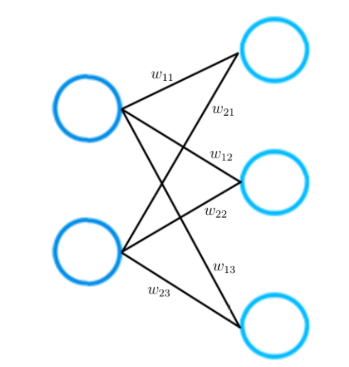
\includegraphics[width=0.5\textwidth]{./slike/weights}
\caption{Veze između neurona [3]}
\label{fig:neuroni-veze}
\end{figure}
%
\\
Na slici $3.1$ svaka veza između dva neurona ima određenu numeričku vrijednost i označena je s w. Prva vrijednost indeksa označava broj neurona u sloju iz kojeg veza potječe, dok druga vrijednost označava broj neurona u sloju do kojeg veza dolazi. Težine između dva sloja mogu se prikazati matricom težina [3]. 
%
\begin{equation}
W =
\begin{pmatrix}
w_{11} & w_{12} & w_{13}\\
w_{21} & w_{22} & w_{23}
\end{pmatrix}
\end{equation}
%
Matrica težina sadrži numeričke vrijednosti za veze između dva sloja neurona u mreži. Dimenzije te matrice odgovaraju broju neurona u dva povezana sloja. Broj redaka odgovara broju neurona u sloju iz kojeg veze potječu, dok broj stupaca odgovara broju neurona u sloju do kojeg te veze vode [3]. 

\newpage
\subsection*{Arhitektura neuronske mreže}

\indent{}
Neuroni su grupirani u komputacijske jedinice koje nazivamo slojevima. Slojevi su međusobno povezani i zajedno čine jedinstvenu strukturu mreže. Neuronske mreže obično se sastoje od $3$ tipa slojeva:
\begin{itemize}
\item[$\bullet$] Ulazni sloj -- prima podatke iz kojih neuronska mreža uči
\item[$\bullet$] Skriveni slojevi -- nalaze se između ulaznog i izlaznog sloja, ovdje se obavljaju svi izračuni u mreži
\item[$\bullet$] Izlazni sloj -- stvara izlaz za zadane ulazne podatke [4]
\end{itemize} 
%
\begin{figure}[!h]
\centering
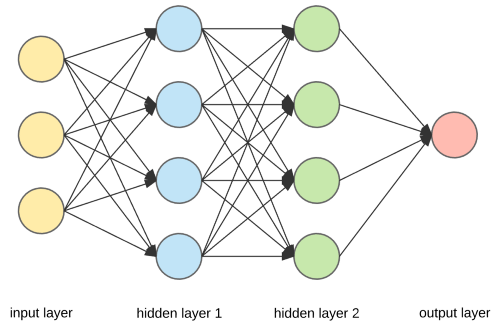
\includegraphics[width=0.8\textwidth]{./slike/net-arch}
\caption{Arhitektura neuronske mreže [4]}
\label{fig:mreza-arh}
\end{figure}
%
Ulazni sloj prima ulazne podatke u obliku vektora značajki $\mathbf{x}$. Ako za primjer uzmemo klasifikaciju slika kože, značajke vektora $\mathbf{x}$ bi predstavljale pojedine piksele u predanim slikama. U ulaznom sloju broj neurona odgovara broju značajki u vektoru $\mathbf{x}$. Izlazni sloj daje vektor predviđanja $\mathbf{y}$ koji predstavlja rezultat do kojeg je neuronska mreža došla. Elementi tog vektora predstavljaju vrijednosti neurona u izlaznom sloju mreže. Za navedeni primjer klasifikacije, svaki neuron u izlaznom sloju predstavljao bi drugačiju klasu, tj. prepoznato kožno oboljenje. Kako bi se taj vektor predviđanja dobio, u skrivenim slojevima potrebno je obaviti određene matematičke operacije [3].
\newpage

\subsection*{Učenje neuronske mreže}

\indent{}
U procesu učenja neuronske mreže, težine između neurona se mijenjaju. Možemo reći da se cjelokupni proces učenja temelji na pronalaženju optimalnih vrijednosti težina među neuronima. Dakako, skup težina koji ćemo htjeti postići razlikovat će se ovisno o početnim ulaznim podatcima i zadatku koji želimo da je mreža u stanju obavljati. U nastavku je opisan proces učenja neuronske mreže [3].\\
\indent{}
Za zadani ulazni vektor značajki $\mathbf{x}$, neuronska mreža računa vektor predviđanja $\mathbf{h}$. Taj korak se naziva i "širenje naprijed" \engl{forward propagation}. Obavljamo produkt ulaznog vektora $\mathbf{x}$ i matrice težina između dva sloja $\mathbf{W}$ [3]. \\
%
\begin{equation}
\begin{split}
\mathbf{x}^T 
\mathbf{W} 
&= 
\begin{pmatrix}
x_{1} & x_{2}
\end{pmatrix}
\begin{pmatrix}
w_{11} & w_{12} & w_{13}\\
w_{21} & w_{22} & w_{23}
\end{pmatrix}
\\
&=
\begin{pmatrix}
x_{1}w_{11} + x_{2}w_{21} & x_{1}w_{12} + x_{2}w_{22} & x_{1}w_{13} + x_{2}w_{23}
\end{pmatrix}
\\
&=
\begin{pmatrix}
z_{1} & z_{2} & z_{3}
\end{pmatrix}
\\
&=
\mathbf{z}
\\
&
\mathbf{h} = \sigma(\mathbf{z})
\end{split}
\end{equation}
 %
\\
Rezultat tog produkta je vektor $\mathbf{z}$, a konačni vektor predviđanja $\mathbf{h}$ dobiva se primjenom tzv. aktivacijske funkcije \engl{activation function} na vektor $\mathbf{z}$. Aktivacijska funkcija u jednadžbi $3.2$ označena je simbolom $\sigma$. U području dubokog učenja najčešće korištene aktivacijske funkcije su $tanh$, $sigmoid$ i $ReLu$. U procesu učenja vrijednosti elemenata vektora $\mathbf{z}$, $\mathbf{h}$ i $\mathbf{y}$ mijenjaju se s promjenama težina u mreži. Ovo opažanje može se proširiti na model neuronske mreže s više slojeva, gdje će se vrijednosti elemenata spomenutih vektora računati za svaki unutarnji sloj mreže [3]. 
%
\begin{figure}[!h]
\centering
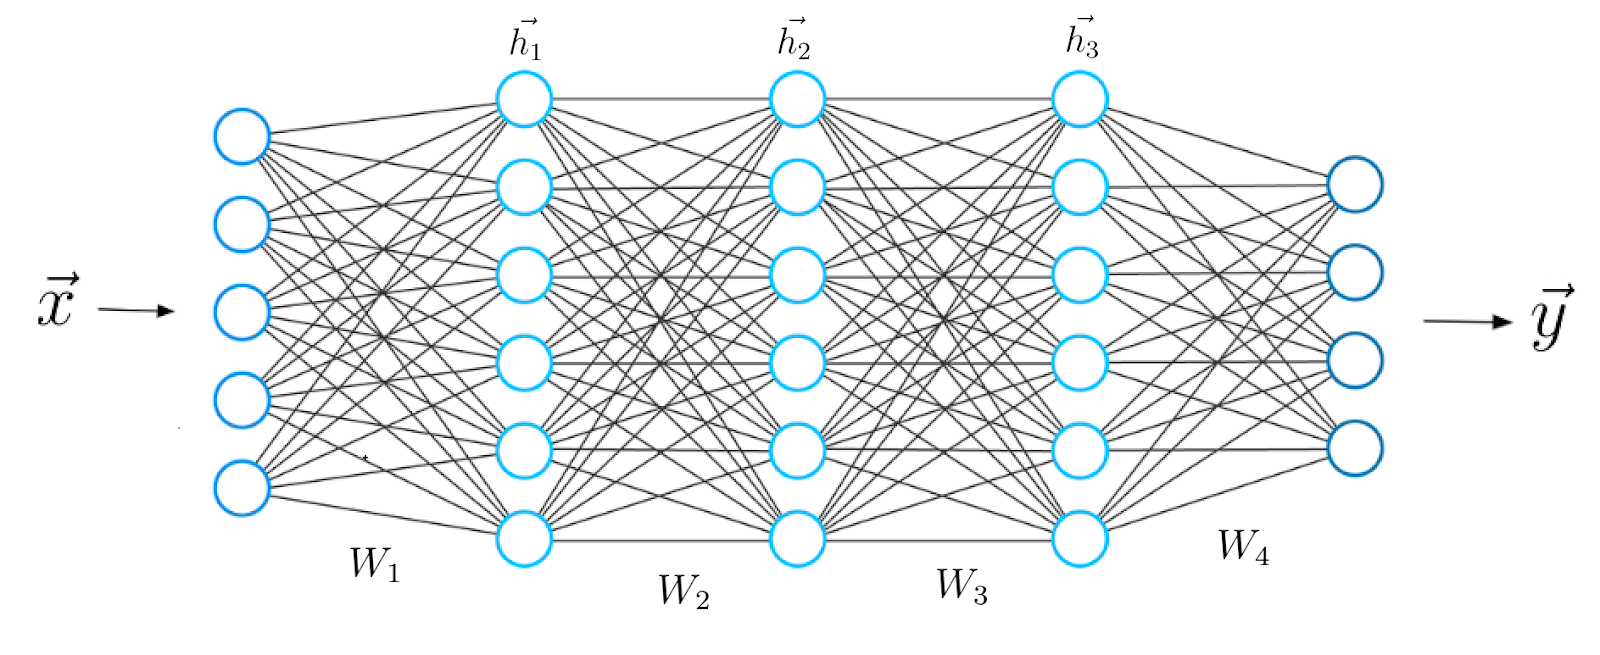
\includegraphics[width=0.95\textwidth]{./slike/deep-net}
\caption{Prikaz vektora u mreži s više slojeva [3]}
\label{fig:dubokamreza}
\end{figure}
%

\subsection*{Funkcija gubitka i gradijentni spust}
\indent{}
Nakon računanja vektora predviđanja neuronske mreže $\mathbf{y}$, on se uspoređuje s vektorom $\mathbf{\hat{y}}$ koji sadrži stvarne vrijednosti kojima su podaci označeni. Vrijednost funkcije gubitka \engl{loss function} ovisi o razlici ova dva vektora. Ta funkcija zapravo daje numeričku ocjenu o točnosti načina na koji model klasificira. Tako minimizacija vrijednosti funkcije gubitka vodi do točnijih predviđanja neuronske mreže. Za dobre rezultate u procesu učenja mreže potrebno je izabrati odgovarajuću funkciju gubitka. Primjer široko prihvaćene funkcije gubitka je funkcija križne entropije \engl{Cross-Entropy Loss function} [3].\\
\begin{equation}
L(\theta) = - \sum_{i=0}^{N} \hat{y}_{i} \cdot \log(y_{i})
\end{equation}
\\
Cilj cijelog procesa učenja neuronske mreže je pronalazak skupa težina za koje je vrijednost funkcije gubitka što je moguće manja. Metoda minimiziranja funkcije gubitka postiže se matematičkom metodom gradijentnog spusta [3].\\
\indent{}
Tijekom gradijentnog spusta, koristi se gradijent funkcije gubitka za korigiranje težina u neuronskoj mreži. 
%
\begin{figure}[!h]
\centering
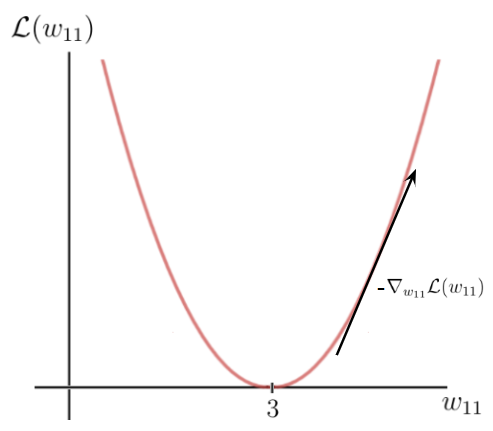
\includegraphics[width=0.6\textwidth]{./slike/gradient}
\caption{Metoda gradijentnog spusta [3]}
\label{fig:gradijent-spust}
\end{figure}
%
\\
Na slici $3.4$ $x$-koordinata prikazuje vrijednost težine $w_{11}$, dok $y$-koordinata prikazuje vrijednosti funkcije gubitka koja ovisi toj težini. Naime, za vrijednost $3$ težine $w$, funkcija gubitka postiže globalni minimum. Računanjem gradijenta te funkcije dobiva se prikazana tangenta koja pokazuje u smjeru najvećeg porasta funkcije gubitka i odgovarajućeg parametra na $x$-osi. Ako se sada taj vektor pomnoži s -$1$, dobiva se smjer najbržeg pada funkcije gubitka, i upravo u tom smjeru se pomiče vrijednost težine $w_{11}$. Ako se tako vrijednosti svih težina u mreži postupno dovedu do minimuma njihovih funkcija gubitka, u konačnici se dobivaju točnije predikcije za ulazni skup podataka [3].  

\section{Konvolucijske neuronske mreže}
\indent{}
Područje računalnog vida jedno je od najatraktivnijih područja u umjetnoj inteligenciji. Za cilj ima omogućiti strojevima da svijet vide kao i ljudi, percipiraju ga na sličan način i koriste stečena znanja kako bi mogli prepoznavati, analizirati i klasificirati slike. Napredak u tom području oslanja se na algoritme dubokog učenja, prvenstveno na algoritam konvolucijskih neuronskih mreža [5]. Upravo konvolucijska neuronska mreža bit će korištena za potrebe klasifikacije spomenutih kožnih oboljenja iz slika kože, no prvo će biti opisana općenita ideja takve mrežne arhitekture.\\
\indent{}
Glavna motivacija za korištenje dubokih neuronskih mreža u području računalnog vida je zaobilaženje dugog postupka izdvajanja značajki. Duboke neuronske mreže sasvim su prikladne za takav zadatak, uzimajući u obzir da kroz slojeve mogu postupno izdvajati značajke ulaznog skupa podataka. Prva pomisao mogla bi biti korištenje potpuno povezanih slojeva \engl{fully connected layer} čiji bi neuroni bili povezani sa svakim od ulaznih piksela, što znači da bi u slučaju crno bijele slike dimenzija 20 x 20 piksela značilo da je jedan neuron povezan s 400 težina, a u slučaju slike u boji s tri panela u boji(crvena, zelena i plava) veličine 200 x  200 piksela s 200 x 200 x 3 = 120 000 težina. To ubrzo dovodi do prevelike složenosti što dovodi do prenaučenosti mreže \engl{overfitting}, tj. mreža će pokazivati dobre rezultate na skupu podataka za učenje, no neće znati klasificirati testne primjere sa zadovoljavajućom točnošću [5].
%
\begin{figure}[!h]
\centering
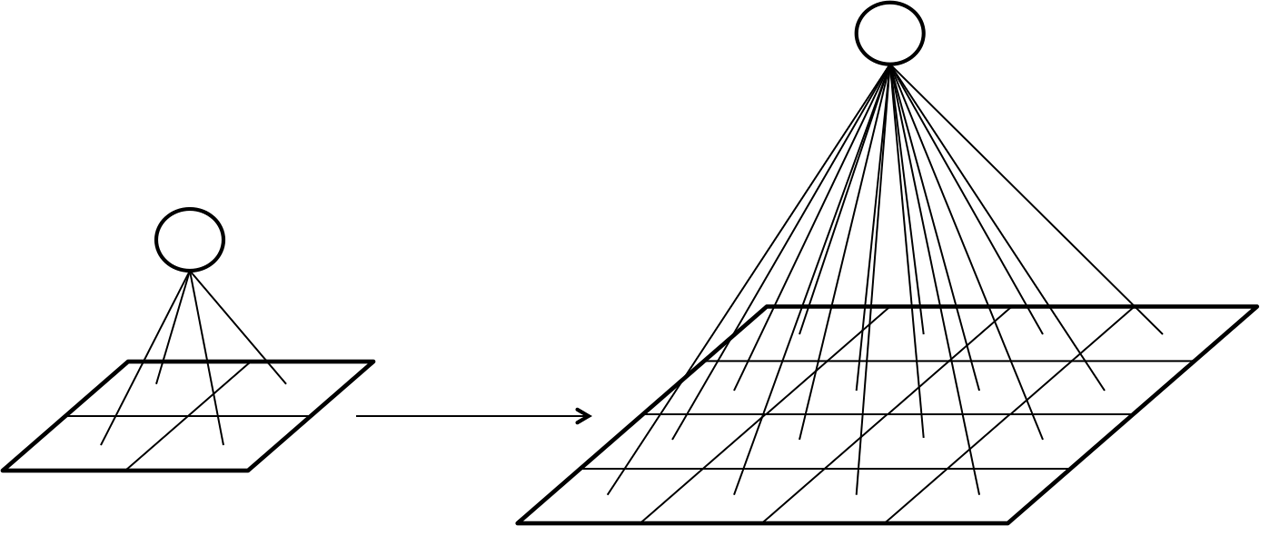
\includegraphics[width=0.7\textwidth]{./slike/conv2}
\caption{Broj veza između slojeva raste povećanjem dimenzija slika [5]}
\label{fig:conv1}
\end{figure}
%
\\
Inspirirani načinom na koji ljudsko oko percipira prostor, slojevi konvolucijske neuronske mreže podijeljeni su u tri dimenzije pa imaju širinu, visinu i dubinu. Neuroni u tim slojevima povezani su samo s manjim dijelom neurona iz prethodnog sloja. Tako konvolucijske neuronske mreže drastično smanjuju broj parametara u mreži te pretvaraju sliku u oblik koji je lakše obraditi, bez gubitka značajki važnih za ispravnu klasifikaciju [5]. To je vrlo važno ako želimo izbjeći problem prenaučenosti, u konačnici dobivamo mrežu koja je stabilna ne samo u klasifikaciji podataka skupa za učenje, nego i novih ulaznih skupova podataka.
%
\begin{figure}[!h]
\centering
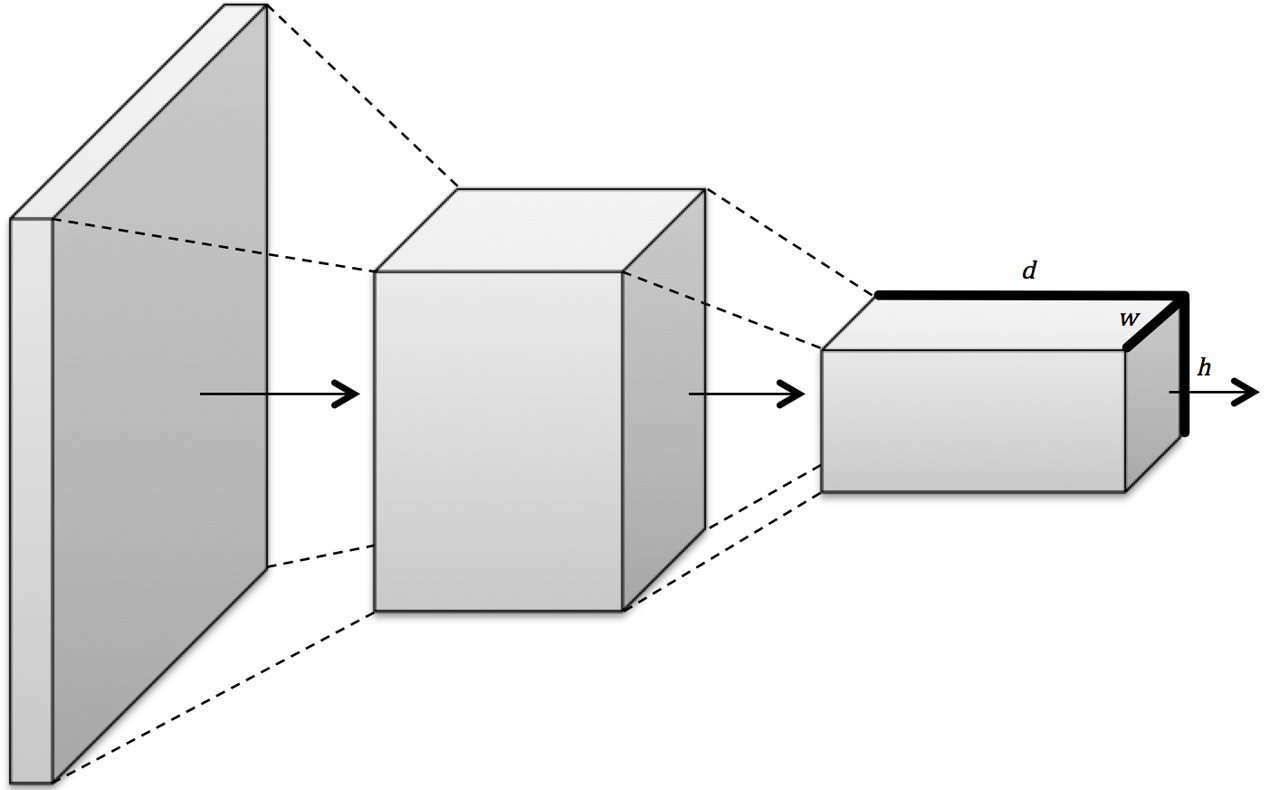
\includegraphics[width=0.8\textwidth]{./slike/conv3}
\caption{Tri dimenzije podataka u slojevima konvolucijske neuronske mreže [5]}
\label{fig:conv2}
\end{figure}
%
\subsection*{Konvolucijski sloj}

Bitan koncept za razvoj konvolucijske mrežne arhitekture je filtar, koji je u osnovi detektor značajki na slici. Postupak konvolucije zasniva se na prolasku filtra određenih dimenzija po cijeloj ulaznoj slici. Tako različiti filtri izdvajaju različite specifične značajke u tzv. mape značajki \engl{feature maps} [5]. Primjenom više filtara, konvolucijska neuronska mreža stvara više mapa značajki i u stanju je uspješno detektirati prostorne i vremenske ovisnosti na slici [7].
%
\begin{figure}[!h]
\centering
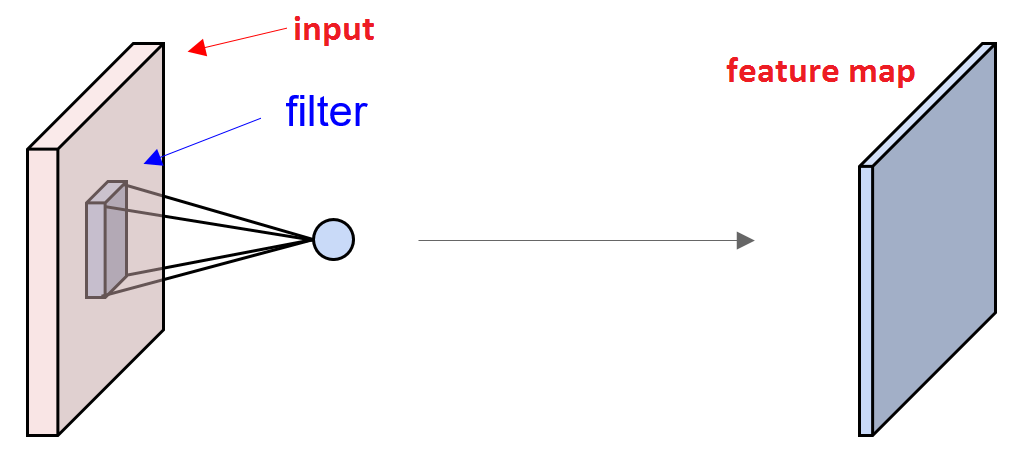
\includegraphics[width=0.85\textwidth]{./slike/conv5}
\caption{Izdvajanje značajki u mapu [6]}
\label{fig:conv4}
\end{figure}
%
\newpage
%
\begin{figure}[!h]
\centering
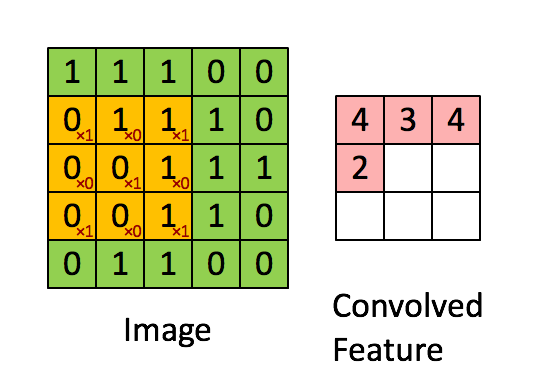
\includegraphics[width=0.75\textwidth]{./slike/conv4}
\caption{Postupak konvolucije [7]}
\label{fig:conv3}
\end{figure}
%
Na slici $3.7$ zelenim poljima prikazana je ulazna slika(I) dimenzija $5$x$5$, dok je žutim poljima prikazan konvolucijski filtar(K) dimenzija $3$x$3$. Rozim poljima prikazana je do tad konstruirana mapa značajki. Kako bi prošao po cijeloj ulaznoj slici filtar se pomiče $9$ puta, pri čemu svaki put obavlja operaciju matričnog množenja između K i dijela slike P nad kojim se u tom trenutku nalazi. Općenito, filtar se pomiče po ulaznoj slici s određenom duljinom koraka \engl{stride length} s lijeva na desno dok ne dođe do ruba slike, kada se pomiče na početak sljedećeg retka. Postupak se ponavlja sve dok se ne prođe cijela površina ulazne slike [7].\\
\indent{}   
U smislu građe konvolucijske neuronske mreže, slojevi neurona predstavljaju izvornu sliku ili mape izdvojenih značajki, dok filtri predstavljaju kombinacije određenih težina među slojevima neurona. Neuron u mapi značajki se aktivira ako filtar zadužen za njegovu aktivnost detektira pojavu tražene značajke u prethodnom sloju neurona [5].\\
%
\begin{figure}[!h]
\centering
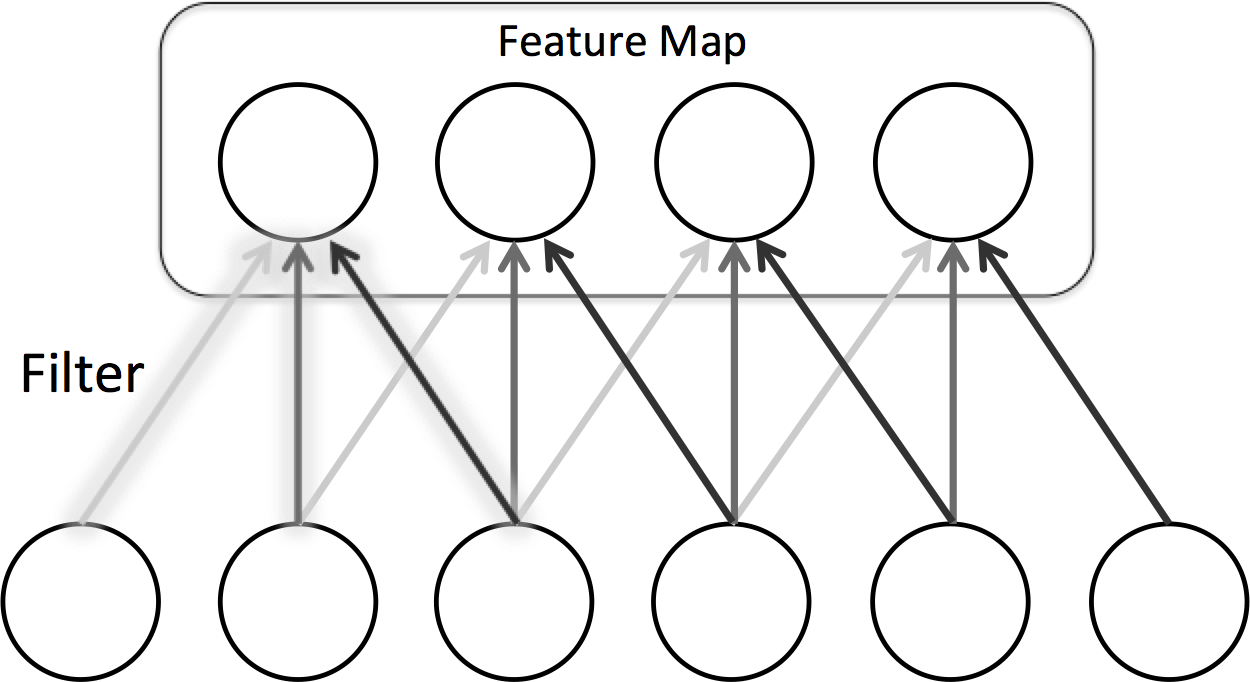
\includegraphics[width=0.75\textwidth]{./slike/conv6}
\caption{Mapa značajki i filtar u konvolucijskoj neuronskoj mreži [5]}
\label{fig:conv5}
\end{figure}
% 
\\
%\indent{}
%Ako se $k$-ta mapa značajki u sloju $m$ ozanačava sa $m^k$, a odgovarajući filter sa vrijednostima svojih težina s W, mape značajki se matematički prikazuju na sljedeći način, ako pretpostavimo da svi neuroni u istoj mapi značajki imaju istu vrijednost bias neurona, $b^k$.[2]\\
%\begin{equation}
% m_{k}^{ij} = f \bigg( (W * x)_{ij} + b^k \bigg)
%\end{equation}
%\\
\indent{}
Filtri u konvolucijskim neuronskim mrežama mogu aktivirati značajke iz svih mapa značajki u određenom sloju, što je od posebne važnosti kod ulaznih slika u boji. Naime, kod takvih slika svaki piksel je prikazan kao kombinacija crvene, zelene i plave \engl{RGB-red, green, blue} pa će se svaka ulazna slika zapravo dijeliti u tri, gdje svaki pojedini dio predstavlja jednu boju. Stoga su mape značajki u 3D obliku, a stvaraju ih 3D filtri koji u ovom slučaju prolaze cijelim volumenom ulazne slike kako bi ih generirali. Konvolucijski sloj sastoji se od skupine filtara pomoću kojih ulazni volumen pretvara u izlazni. Dubina filtra odgovara dubini ulazne slike, tako da filtar može kombinirati informacije o svim naučenim značajkama. Dubina izlaznog volumena konvolucijskog sloja odgovara broju filtara u tom sloju, jer svaki filtar stvara svoj vlastiti izlazni volumen [5].\\

\indent{}
Zadaća konvolucijskog sloja je izdvajanje značajki visoke razine iz ulazne slike. Konvolucijske neuronske mreže obično imaju više ovakvih slojeva. Prvi konvolucijski sloj iz ulazne slike izdvaja značajke niske razine kao što su rubovi, boja i orijentacija gradijenta. Daljnji slojevi sve se više prilagođavaju značajkama više razine, stvarajući u konačnici mrežu koja je u stanju analizirati i klasificirati slike s visokom točnošću [7]. 

\newpage
%
\begin{figure}[!h]
\centering
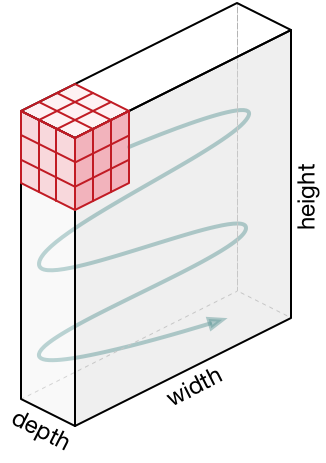
\includegraphics[width=0.3\textwidth]{./slike/conv8}
\caption{Skica prolaza 3D filtra cijelim volumenom ulazne slike [7]}
\label{fig:conv7}
\end{figure}
%
\begin{figure}[!h]
\centering
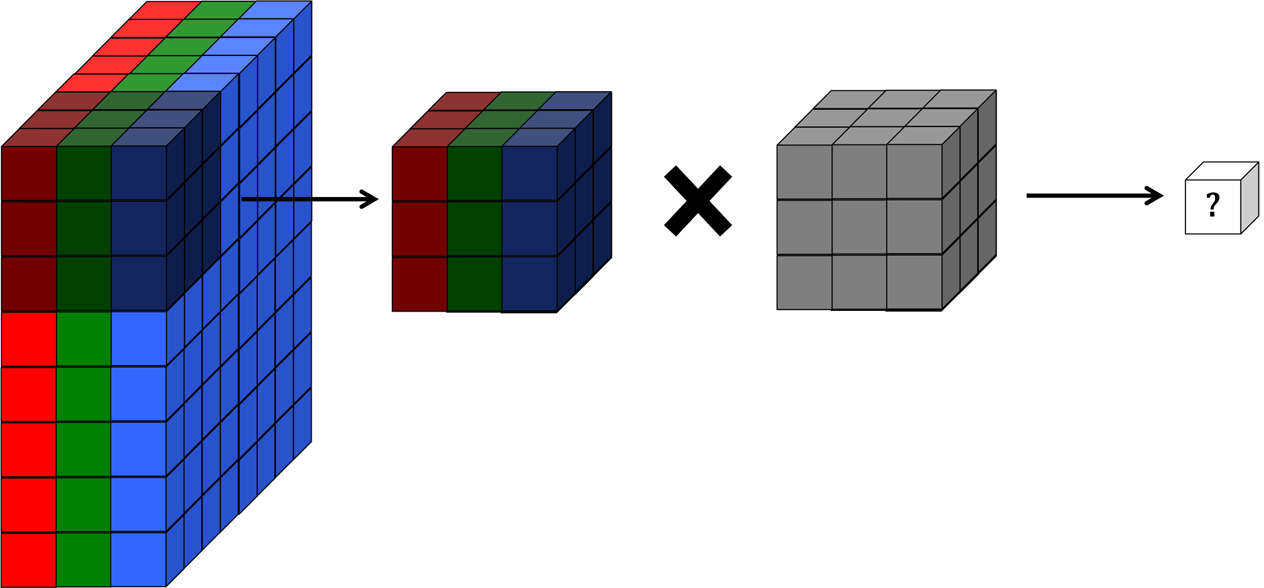
\includegraphics[width=0.85\textwidth]{./slike/conv7}
\caption{Primjena 3D filtra na ulaznu RGB sliku u 3D formatu [5]}
\label{fig:conv6}
\end{figure}
% 
\begin{figure}[!h]
\centering
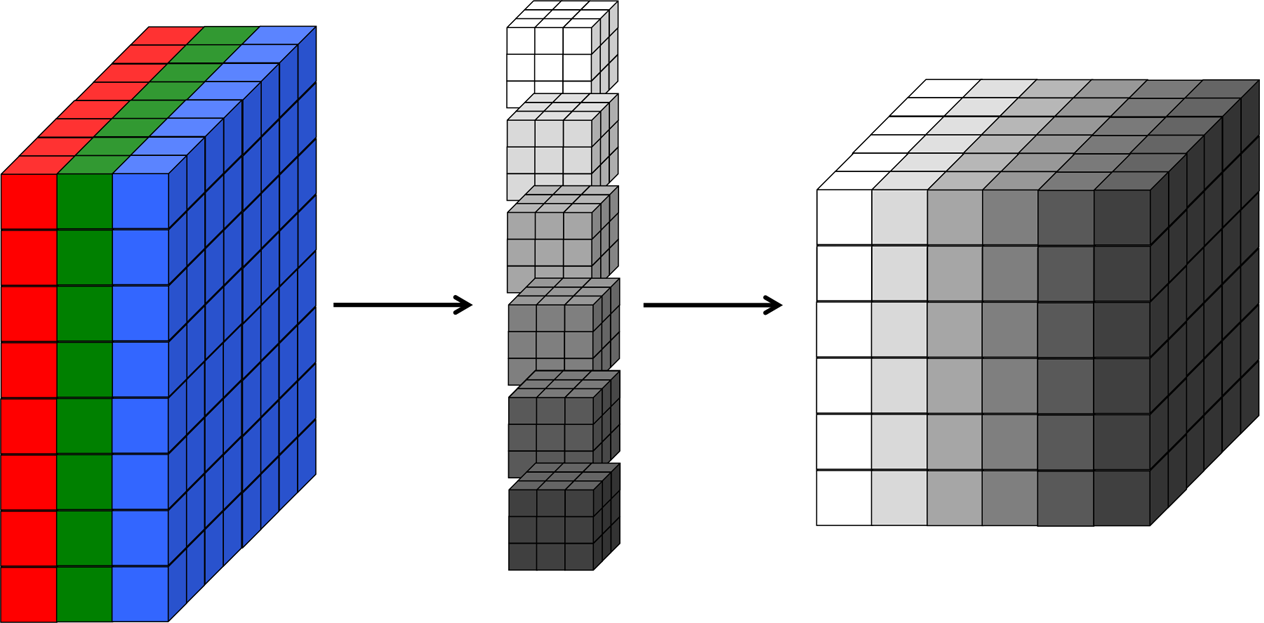
\includegraphics[width=0.85\textwidth]{./slike/conv9}
\caption{Obrada ulazne 3D slike konvolucijskim slojem [5]}
\label{fig:conv6}
\end{figure}
% 
\newpage

\subsection*{Sloj sažimanja}

Sloj sažimanja \engl{pooling layer} uobičajeno je koristiti nakon konvolucijskih slojeva kako bi se smanjila prostorna složenost stvorenih mapa značajki. Smanjenjem dimenzionalnosti podataka u mreži smanjuje se vrijeme i količina računalnih resursa potrebna za njihovu obradu, što je važno u procesu učenja mreže. Glavna ideja iza sloja sažimanja je razlomiti mapu značajki na jednake cjeline i potom za svaku od cjelina generirati jedno polje u sažetoj mapi značajki, što značajno utječe na smanjenje broja parametara u mreži. Ovakav postupak iz mapa značajki dodatno izdvaja one najdominantnije, čime u konačnici stvaramo veće šanse za izgradnju robusnijeg modela koji će biti manje sklon problemu prenaučenosti [7].
% 
\begin{figure}[!h]
\centering
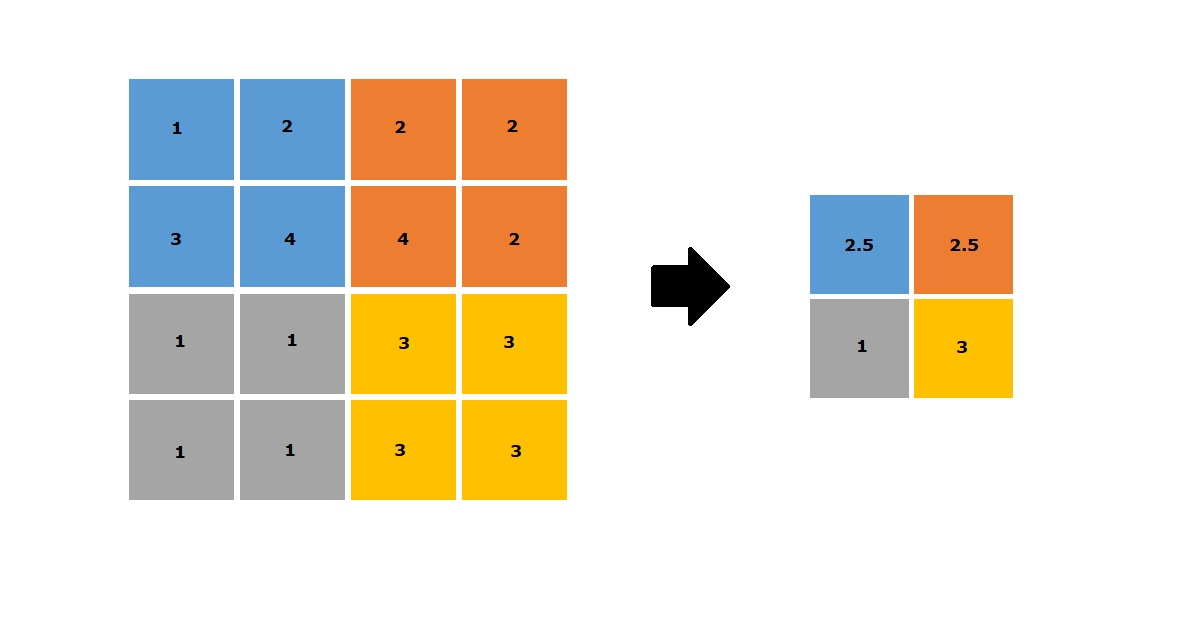
\includegraphics[width=1\textwidth]{./slike/pooling}
\caption{Primjena sloja sažimanja na generiranoj mapu značajki}
\label{fig:pooling1}
\end{figure}
%
\\
Postoje dvije vrste sloja sažimanja:
\begin{itemize}
\item[$\bullet$] Sažimanje maksimalnom vrijednosti(eng. max pooling) -- iz cjeline u mapi značajki izdvaja se maksimalna vrijednost
\item[$\bullet$] Sažimanje srednjom vrijednosti(eng. average pooling) -- iz cjeline u mapi značajki izdvaja se srednja vrijednost [7]
\end{itemize}
%
Sažimanje maksimalnom vrijednošću uz smanjenje dimenzionalnosti u potpunosti uklanja bučne aktivacije u mapi značajki, dok sažimanje srednjom vrijednosti obavlja samo smanjenje dimenzionalnosti. Stoga sažimanje maksimalnom vrijednošću općenito daje bolje rezultate u procesu učenja [7].
\newpage

% 
\begin{figure}[!h]
\centering
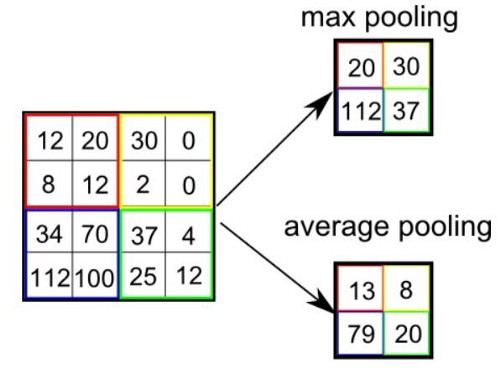
\includegraphics[width=0.6\textwidth]{./slike/pooling1}
\caption{Sažimanje maksimalnom i srednjom vrijednošću [7]}
\label{fig:pooling1}
\end{figure}
%

\subsection*{Potpuno povezani sloj}

Potpuno povezani slojevi \engl{fully connected layers} čine nekoliko zadnjih slojeva konvolucijske neuronske mreže. Ulaz u neurone potpuno povezanog sloja je izlaz iz zadnjeg konvolucijskog ili sloja sažimanja, na koji je dodan sloj neurona za izravnavanje \engl{flatten layer}. Sloj za izravnavanje izlaz iz konvolucijskog ili sloja sažimanja u obliku trodimenzionalne matrice pretvara u jednodimenzionalni vektor [7]. 
% 
\begin{figure}[!h]
\centering
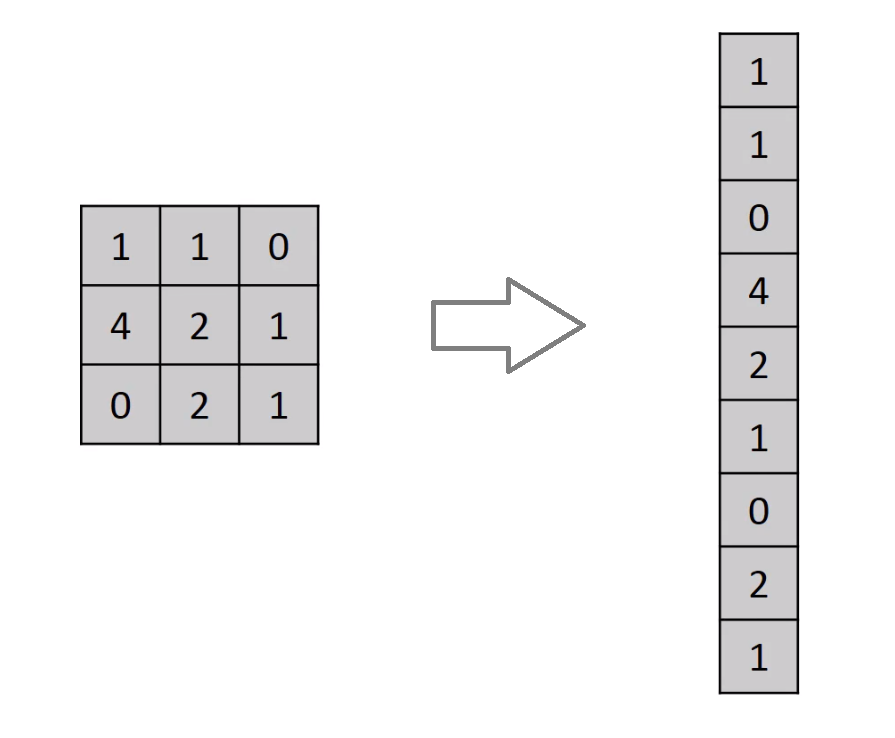
\includegraphics[width=0.6\textwidth]{./slike/flatten}
\caption{Primjena sloja za izravnavanje prije potpuno povezanog sloja [7]}
\label{fig:flatten}
\end{figure}
%
\\
Ovakav jednodimenzionalni vektor dalje je povezan s nekoliko potpuno povezanih slojeva. U njima se obavljaju svi izračuni karakteristični za potpuno povezane neuronske mreže, uz korištenje $ReLu$ aktivacijske funkcije. Posljednji potpuno povezani sloj potom koristi $Softmax$ aktivacijsku funkciju pomoću koje se na izlazu iz mreže dobivaju vjerojatnosti pripadnosti ulazne slike jednoj od klasa. Na taj se način konvolucijske neuronske mreže koriste za potrebe klasifikacije [16]. Na sljedećoj slici prikazana je uobičajena arhitektura konvolucijske neuronske mreže koja se sastoji od nekoliko uzastopnih slojeva konvolucije i sažimanja, nakon kojih dolazi sloj za izravnavanje i nekoliko potpuno povezanih slojeva. U ovom slučaju riječ je o neuronskoj mreži za potrebe klasifikacije slika s prijevoznim sredstvima.
% 
\begin{figure}[!h]
%\centering
\hspace{-0.05\textwidth}
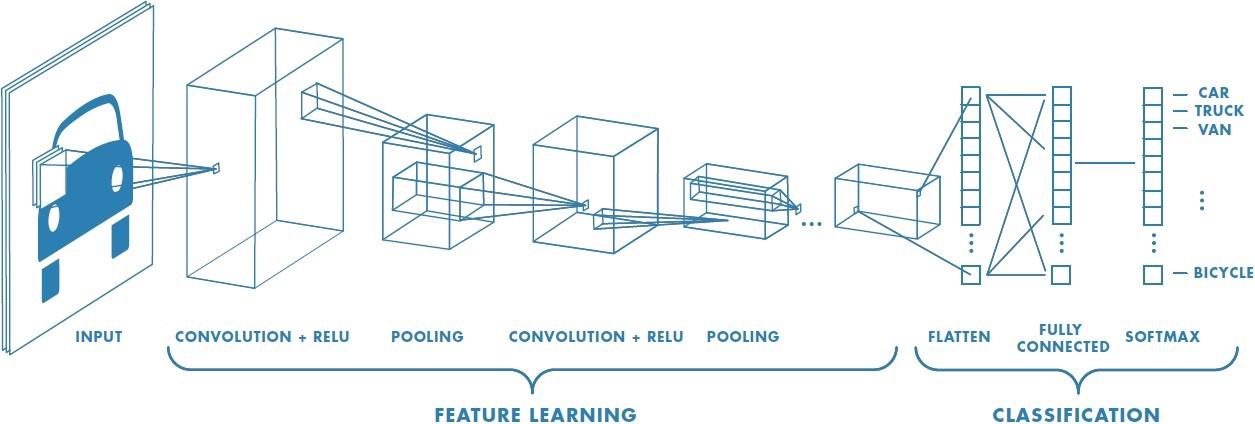
\includegraphics[width=1.1\textwidth]{./slike/convolutionnet}
\caption{Uobičajena arhitektura konvolucijske neuronske mreže [7]}
\label{fig:conv-arch}
\end{figure}
%

\chapter{Izgradnja modela duboke neuronske mreže}
Kao što je već spomenuto u uvodnom dijelu, cilj je izgradnja modela duboke neuronske mreže koja će moći klasificirati kožna oboljenja temeljem slika kože. U idućim potpoglavljima bit će opisan postupak razvoja i implementacije takvog modela.
\section{Korištene tehnologije i alati}
\indent{}
Za potrebe implementacije modela korišten je programski jezik Python i vanjske biblioteka Keras, NumPy i Pandas. Keras je Python biblioteka otvorenog koda \engl{open source} za razvoj i evaluaciju modela dubokog učenja. Služi kao sučelje za numeričku komputacijsku Python biblioteku TensorFlow i omogućava pojednostavljenu definiciju i učenje modela dubokih neuronskih mreža [17]. NumPy je Python biblioteka koja pojednostavljuje rad s n-dimenzionalnim poljima što je od velike važnosti pri manipulaciji velikim količinama podataka korištenim za modele dubokog učenja [18]. Pandas je Python biblioteka otvorenog koda korištena za analizu i učitavanje podataka, a razvijena je kao dio NumPy biblioteke [19].\\ 
\indent{}
Za učenje i razvoj modela duboke neuronske mreže korištena je platforma Google Colab koja osim pisanja i izvođenja Python koda izravno u browseru nudi i besplatan pristup dodatnoj hardverskoj potpori za potrebe učenja neuronskih mreža. 
\newpage
\section{Podaci}
\indent{}
Prvi korak je prikupljanje prikladnih podataka, tj. slika kože pomoću kojih će model učiti. Za ovaj zadatak odabran je $HAM10000$ \engl{"Human Against Machine with $10000$ training images"} skup podataka koji se sastoji od $10015$ slika kožnih lezija. Taj skup podataka je javan, a objavio ga je "Harvard database" u lipnju 2018. godine. Više od 50\% lezija potvrđene su histopatologijom(histo), istinita oznaka za ostala oboljenja \engl{ground truth} temelji se na naknadnim dermatološkim pregledima(follow\_up), konsenzusu stručnjaka(konsenzus) ili potvrdi in-vivo konfokalnom mikroskopijom(confocal) [15].\\
\indent{}
U dijelu 2.2 opisane su sve klase kožnih oboljenja koja su prisutna u skupu podataka. Kratice klasa tih oboljenja korištene u datoteci s metapodacima su sljedeće:

\begin{enumerate}
\item Melanocytic nevi -- nv
\item Melanoma -- mel
\item Benign keratosis-like lesions -- bkl
\item Basal cell carcinoma -- bcc
\item Actinic keratoses -- akiec
\item Vascular lesions -- vas
\item Dermatofibroma -- df
\end{enumerate}

\subsection*{Metapodaci}

Uz slike kožnih oboljenja, u skupu podataka $HAM10000$ priložena je i datoteka s metapodacima $HAM10000\_metadata.csv$. U toj datoteci priložene su dodatne informacije o skupu podataka. Najvažniji podatak za potrebe izgradnje klasifikacijskog modela svakako je oznaka klase kožnog oboljenja za svaku sliku. Ostali metapodaci neće biti od tolike važnosti za samu klasifikaciju, no svakako ih valja proučiti kako bi se stekao bolji dojam o prirodi podataka koji će se koristiti za izgradnju modela. U nastavku je dan uvid u strukturu metapodataka dostupnih u navedenoj datoteci.
\newpage
%  
\begin{figure}[!h]
\centering
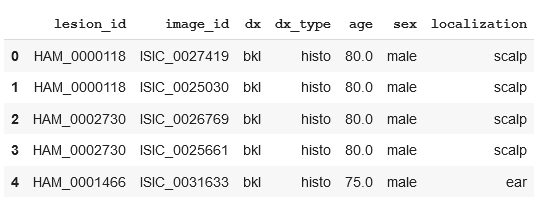
\includegraphics[width=0.9\textwidth]{./slike/colab1}
\caption{Metapodaci iz datoteke $HAM10000\_metadata.csv$}
\label{fig:colab1}
\end{figure}
%
\indent{}
U metapodacima su značajni stupci koji označavaju kraticu klase kožne lezije(dx), tip istinite oznake za oboljenje(dx\_type), godine(age) i spol(sex) bolesnika te lokalizacija lezije na tijelu(localization). Stupac za id slike(image\_id) bit će korišten za stvaranje putanje do slike oboljenja u učitanim podacima.\\
\indent{}
Korištenjem ovih metapodataka moguće je podrobnije istražiti osobine promatranog skupa podataka. Kao što je već spomenuto, u konkretnom klasifikacijskom modelu koristit će se samo podatak o klasi kožne lezije, no ostale metapodatke moguće je iskoristiti za daljnje studije vezane za proučavanje populacije. U nastavku su prikazane raspodjele podataka po dostupnim metapodacima.
%\newpage
%
\begin{figure}[!h]
\hspace{-0.1\textwidth}
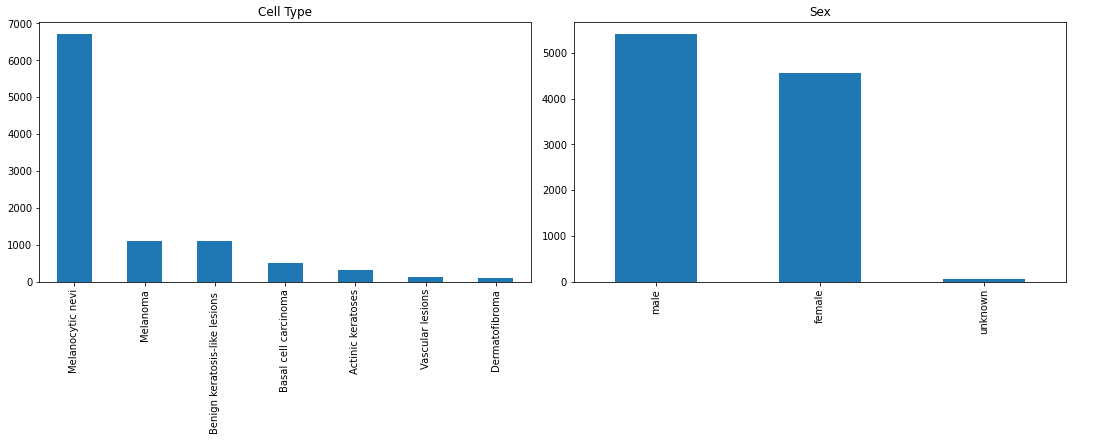
\includegraphics[width=1.2\textwidth]{./slike/colab2}
\caption{Distribucija klasa kožnih lezija i spola pacijenata u skupu podataka}
\label{fig:colab2}
\end{figure}
\\
%
Iz prikazane distribucije po klasama kožnih lezija vidljivo je da postoji velik disbalans u broju slika po pojedinoj klasi. Prisutno je 6705 slika oboljenja klase "Melanocytic nevi", dok slika oboljenja klase "Dermatofibroma" ima svega 115. Ovakve pojave su vrlo česte u skupovima podataka za medicinska istraživanja zbog ograničenog broja pacijenata i učestalosti pojavljivanja određene bolesti u promatranoj populaciji.\\
%
\begin{figure}[!h]
\hspace{-0.1\textwidth}
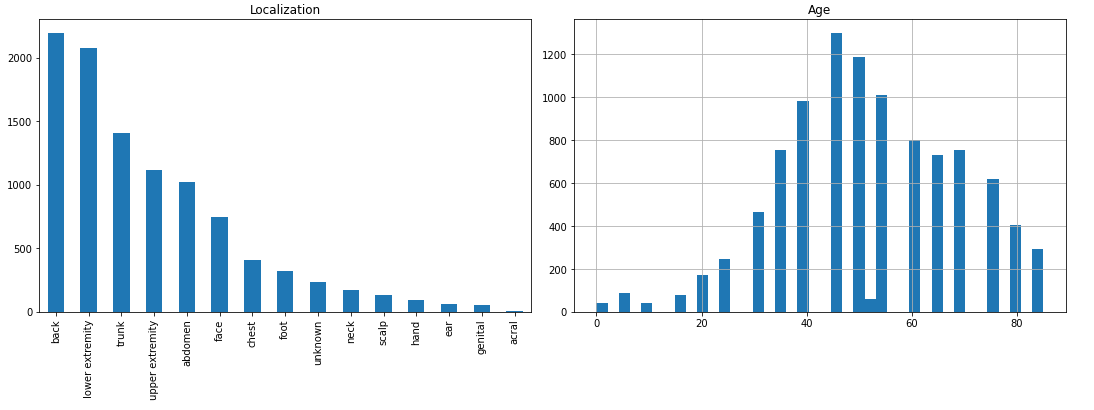
\includegraphics[width=1.2\textwidth]{./slike/colab3}
\caption{Distribucija lokalizacija kožinih lezija i starosti pacijenata u skupu podataka}
\label{fig:colab3}
\end{figure}
%
\\
Iz prikazanih distribucija po fizičkoj lokalizaciji kožnih lezija vidljivo je da se najčešće javljaju na leđima i nogama, a iz distribucije starosti promatranih pacijenata da su najčešće u srednjoj životnoj dobi.

\section{Priprema podataka}

%dodati jos sa kagglea

Nakon preuzimanja i raspakiravanja zip arhive s bazom podataka o kožnim oboljenjima, potrebno je obaviti učitavanje i pretprocesiranje podataka kako bi se mogli koristiti u gradnji klasifikacijskog modela.

\subsection*{Učitavanje slika u Dataframe}
Nakon učitavanja datoteke s metapodacima($HAM10000\_metadata.csv$) Pandas bibliotekom, kao povratnu vrijednost dobivamo Pandas Dataframe. Dataframe omogućava lakše baratanje dvodimenzionalnim tabličnim podacima s označenim redovima i stupcima, a dodatno je omogućena promjena i dodavanje podataka u Dataframe [19]. Učitavanje datoteke postižemo navedenom naredbom.

\begin{minted}[breaklines]{python}
skin_dataframe = pd.read_csv(os.path.join(base_skin_dir, 'HAM10000_metadata.csv'))
\end{minted}

U učitani dataframe potrebno je dodati dva stupca. Stupac $cell\_type$ u kojemu će za svaku sliku biti oznaka punog imena kožne lezije generira se pomoću kratice lezije($dx$) i Python rječnika \engl{dictionary} $lesion\_type\_dict$.   Stupac $cell\_type\_index$ će za svaku sliku pohranjivati indeks pripadajuće oznake kožne lezije u Python rječniku $lesion\_type\_dict$, što će nam pomoći pri baratanju podacima u kasnijim koracima. Rječnik $lesion\_type\_dict$ i naredba za dodavanje navedenih stupaca u Dataframe dani su u nastavku.

\begin{minted}[breaklines]{python}
lesion_type_dict = {
    'nv': 'Melanocytic nevi',
    'mel': 'Melanoma',
    'bkl': 'Benign keratosis-like lesions ',
    'bcc': 'Basal cell carcinoma',
    'akiec': 'Actinic keratoses',
    'vasc': 'Vascular lesions',
    'df': 'Dermatofibroma'
}

skin_dataframe['cell_type'] = skin_dataframe['dx'].map(lesion_type_dict.get) 
skin_dataframe['cell_type_index'] = pd.Categorical(skin_dataframe['cell_type']).codes
\end{minted}

Idući korak je dodavanje stupca sa slikama($image$) u Dataframe, no prije toga potrebno je dodati još jedan stupac($path$) u kojem će za svaku sliku biti zapisana pripadajuća putanja na disku. Putanja pojedine slike dobiva se iz prethodno pripremljenog Python rječnika $imageid\_path\_dict$, gdje su parovi ključ:vrijednost oblika image\_id:putanja.\\
%
\begin{figure}[!h]
\hspace{-0.05\textwidth}
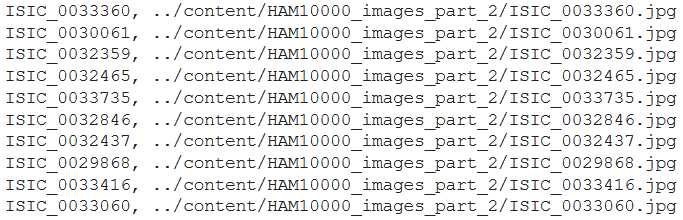
\includegraphics[width=1.1\textwidth]{./slike/dict}
\caption{Dio sadržaja rječnika $imageid\_path\_dict$}
\label{fig:dict}
\end{figure}
%
\\ 
Slike su originalno spremljene u $.jpg$ formatu dimenzija $450$x$600$x$3$, što nije prikladno za ulaz u Keras model duboke neuronske mreže. Iz tog razloga slikama se dimenzije mijenjaju na $100$x$75$. Konačno, dodavanje stupca $image$ u Dataframe uz učitavanje i promjenu veličine slika prikazano je u nastavku.

\begin{minted}[breaklines]{python}
skin_dataframe['image'] = skin_dataframe['path'].map(lambda x:np.asarray(Image.open(x).resize((100,75))))
\end{minted}
%
\begin{figure}[!h]
\hspace{-0.1\textwidth}
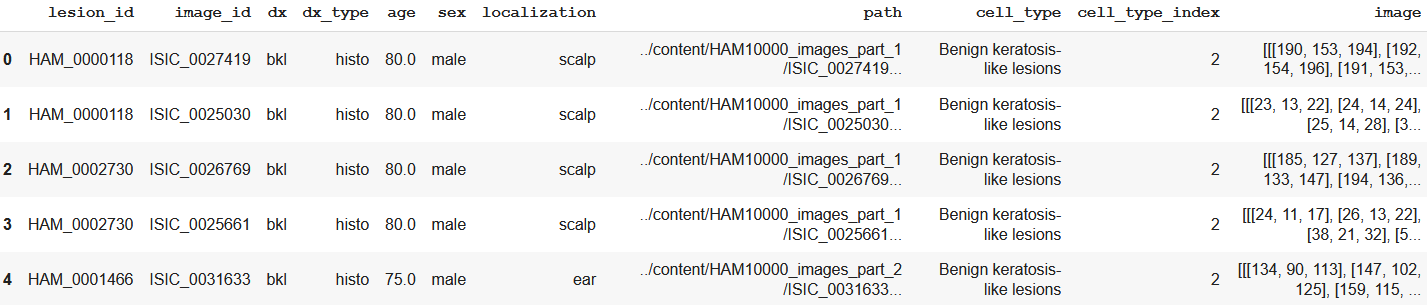
\includegraphics[width=1.2\textwidth]{./slike/dataframe}
\caption{Dataframe sa dodanim stupcima $cell\_type$, $cell\_type\_index$, $path$ i $image$}
\label{fig:dataframe}
\end{figure}
%

\subsection*{Podjela podataka na značajke i ciljne oznake}
Još jedan međukorak je izdvajanje ciljnih oznaka učitanih podataka. Stupac $cell\_type\_index$ izdvaja se iz Dataframe-a i sprema u polje ciljnih oznaka $target$, dok polje značajki $features$ čine preostali stupci. To postižemo idućim naredbama.

\begin{minted}[breaklines]{python}
features=skin_dataframe.drop(columns=['cell_type_index'],axis=1)
target=skin_dataframe['cell_type_index']
\end{minted}

\subsection*{Transformacija ciljnih oznaka}

Polje ciljnih oznaka $target$ potrebno je pretvoriti u zapis $One$ $Hot$ $Encoding$. Takav zapis uklanja cjelobrojnu oznaku i zamjenjuje ju binarnom ovisno o broju mogućih vrijednosti. Kako u promatranom skupu podataka postoji $7$ klasa kožnih oboljenja, oznake će biti duljine $7$ binarnih znakova.

\begin{minted}[breaklines]{python}
y_train = to_categorical(y_train_o, num_classes = 7)
y_test = to_categorical(y_test_o, num_classes = 7)
\end{minted}

\subsection*{Stvaranje setova za učenje i testiranje}
Kako bi se podaci pripremili za implementaciju modela potrebno ih je podijeliti u skupove za učenje, validaciju i testiranje. Model uči na skupu podataka za učenje, određuje optimalne parametre na skupu podataka za validaciju te se testira s određenim optimalnim parametrima na skupu podataka za testiranje. Podjela inicijalnog skupa podataka na ova tri skupa napravljena je u omjeru 72\%/8\%/20\%. 

\begin{minted}[breaklines]{python}
x_train_o, x_test_o, y_train_o, y_test_o = train_test_split(features, target, test_size=0.20,random_state=555)

x_train, x_validate, y_train, y_validate = train_test_split(x_train, y_train, test_size = 0.1, random_state = 55)
\end{minted}


\section{Gradnja modela}

Model duboke neuronske mreže izgrađen je prema načelima konvolucijske mrežne arhitekture, koja je prethodno teorijski opisana u poglavlju 3.2. Korišten je Keras Sequential API [17] koji omogućava apstrahiranu gradnju mreže sloj po sloj. Na početku se nalazi ulazni \engl{input} sloj za učitavanje podataka, dimenzija $75$x$100$x$3$. Slijede tri sloja konvolucije. Prvi se sastoji od jednog konvolucijskog sloja i sloja sažimanja, a druga dva od dva konvolucijska sloja nakon kojih dolazi sloj sažimanja. Kao optimalna veličina filtra u konvolucijskim slojevima pokazala se veličina $3$x$3$, a u slojevima sažimanja korišteno je sažimanje maksimalnom vrijednošću s veličinom površine sažimanja $2$x$2$. Nakon konvolucijskih slojeva primijenjen je sloj za izravnavanje i $3$ potpuno povezana sloja s aktivacijskom funkcijom $ReLu$. Zadnji sloj je izlazni s aktivacijskom funkcijom $Softmax$. 
\newpage
%
\begin{figure}[!h]
%\hspace{-0.1\textwidth}
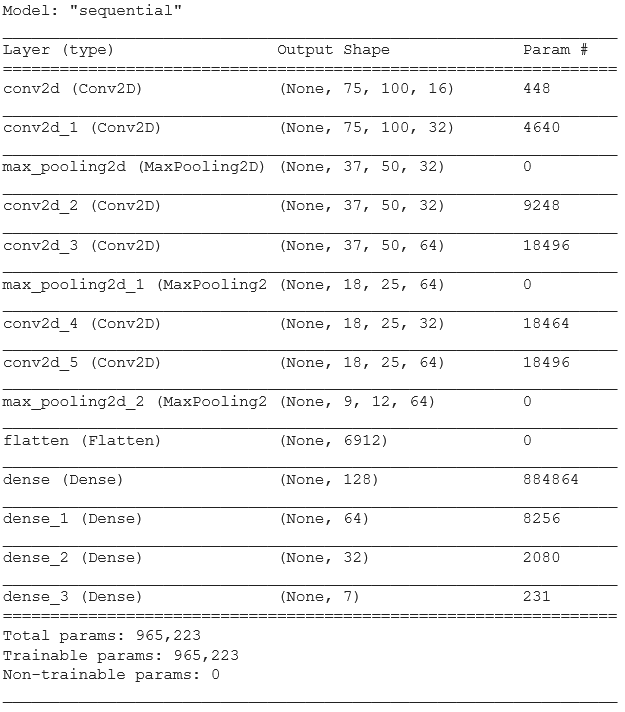
\includegraphics[width=1\textwidth]{./slike/netmodel}
\caption{Izgrađeni model}
\label{fig:netmodel}
\end{figure}
%

\section{Učenje i testiranje modela}

Prije pokretanja procesa učenja, potrebno je definirati optimizacijsku funkciju \engl{optimizer}, funkciju gubitka \engl{loss function} i mjeru kojom ćemo tijekom učenja pratiti performanse modela \engl{metrics}. Optimizacijska funkcija iterativno mijenja vrijednosti parametara u neuronskoj mreži u cilju smanjivanja vrijednosti funkcije gubitka. Korištena je $Adam$ optimizacijska funkcija jer održava pojedinačne stope učenja po parametru u neuronskoj mreži. Funkcija gubitka mjeri koliko dobro model predviđa označene podatke i mjeri stopu greške između stvarnih i predviđenih oznaka. Za probleme klasifikacija s više od dvije klase koristi se funkcija gubitka kategoričke križne entropije \engl{categorical\_crossentropy}. Za mjeru učinkovitosti korištena je preciznost predviđanja modela na validacijskom setu podataka \engl{accuracy}. 

\begin{minted}[breaklines]{python}
optimizer = Adam(learning_rate=0.001, beta_1=0.9, beta_2=0.999, epsilon=None, decay=0.0, amsgrad=False)

model.compile(optimizer = optimizer , loss = "categorical_crossentropy", metrics=["accuracy"])
\end{minted}

Bitan pojam je i stopa učenja \engl{learning rate} koja je mjera brzine kojom optimizacijska funkcija mijenja parametre modela. Što je stopa učenja veća optimizacijska funkcija za veću stopu mijenja parametre, što može dovesti do upadanja u lokalni minimum funkcije gubitka. Pokazalo se da je korisno postupno smanjivati stopu učenja. To se postiže uporabom funkcije $ReduceLROnPlateau$ iz paketa $Keras.Callbacks$ [17], ta funkcija smanjuje stopu učenja za pola ako se preciznost modela ne povećava nakon tri epohe. 

\begin{minted}[breaklines]{python}
lr_reduction = ReduceLROnPlateau(monitor='val_accuracy', 
                                 patience=3, 
                                 verbose=1, 
                                 factor=0.5, 
                                 min_lr=0.00001)
\end{minted}

Konačno, možemo pokrenuti proces učenja, a potom i testiranja modela.
%
\begin{figure}[!h]
\hspace{-0.1\textwidth}
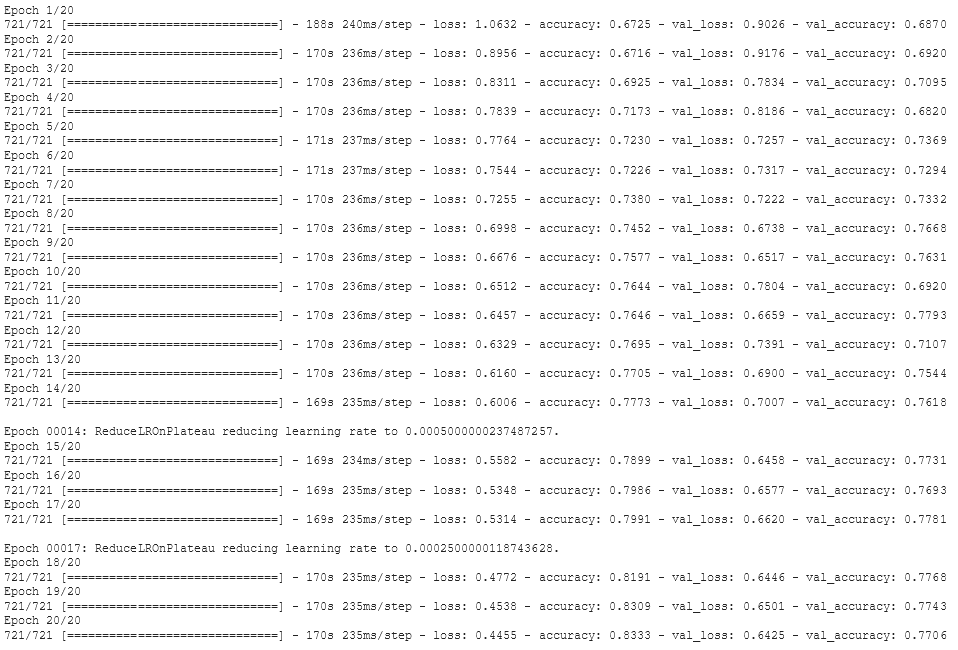
\includegraphics[width=1.2\textwidth]{./slike/colab4}
\caption{Proces učenja modela}
\label{fig:colab4}
\end{figure}
%
\newpage
%
\begin{figure}[!h]
\hspace{-0.05\textwidth}
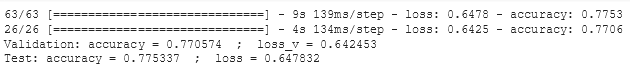
\includegraphics[width=1.1\textwidth]{./slike/colab5}
\caption{Proces testiranja modela}
\label{fig:colab5}
\end{figure}
%

Proces učenja sastoji se od 20 epoha, a veličina uzorka \engl{batch size} je 10. Model postiže konačnu točnost od 88.33\% na skupu podataka za učenje, 77.06\% na skupu podataka za validaciju i 77.0574\% na skupu podataka za testiranje.
\newpage
\section{Usboredba sa sličnim rješenjima}

\subsection*{ResNet50}

Ideja iza rezidualnih mreža(ResNet) je pokušaj prevladavanja problema pri radu s dubljim modelima gdje se pogreška u učenju počinje povećavati s dodavanjem dodatnih slojeva. Ova mrežna arhitektura najčešće je korištena unaprijed naučena mreža za prepoznavanje slika. Model $ResNet50$ koji koristi 50 konvolucijskih slojeva na promatranom skupu podataka postigao je navedene točnosti [8].
%
\begin{figure}[!h]
\centering
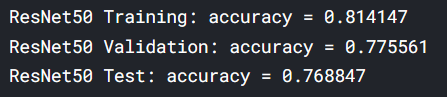
\includegraphics[width=0.7\textwidth]{./slike/resnet}
\caption{Postignute točnosti modela $ResNet50$ [8]}
\label{fig:resnet}
\end{figure}
%
\\
Iako su postignute sličnosti slične onima u razvijenom modelu, model $ResNet50$ imao je manju standardnu devijaciju nakon nekoliko uzastopnih procesa učenja [8].


\chapter{Izgradnja aplikacije}
Nakon izgradnje modela duboke neuronske mreže bilo je potrebno izgraditi mobilnu aplikaciju koja će pružiti korisničko sučelje za klasifikaciju kožnih oboljenja na temelju slika kože. U idućim potpoglavljima bit će opisan postupak razvoja i implementacije takve aplikacije.

\section{Opis sustava}
Aplikacija omogućava slikanje kože i prijenos slika na poslužiteljsku stranu gdje se obavlja klasifikacija kožnog oboljenja korištenjem razvijenog modela duboke neuronske mreže. Nakon klasifikacije rezultati se s poslanom slikom spremaju u bazu podataka. Kako se rezultati trajno pohranjuju u bazu podataka, korisniku je u aplikaciji omogućen ispis svih obavljenih klasifikacija. Osim uporabe kamere, omogućen je i izbor iz galerije za odabir postojeće slike za klasifikaciju. Kako bi korisnik mogao pristupiti opisanim funkcionalnostima potrebna je njegova registracija i prijava u sustav, pri čemu se podaci o korisniku također trajno pohranjuju u bazu podataka. 

\section{Arhitektura sustava}
Sustav je oblikovan u REST arhitekturalnom stilu i ima tri glavna sudionika: korisničku stranu \engl{frontend}, poslužiteljsku stranu \engl{backend} i bazu podataka \engl{database}. Skica arhitekture razvijenog sustava prikazana je na sljedećoj slici.
\newpage
%
\begin{figure}[!h]
\centering
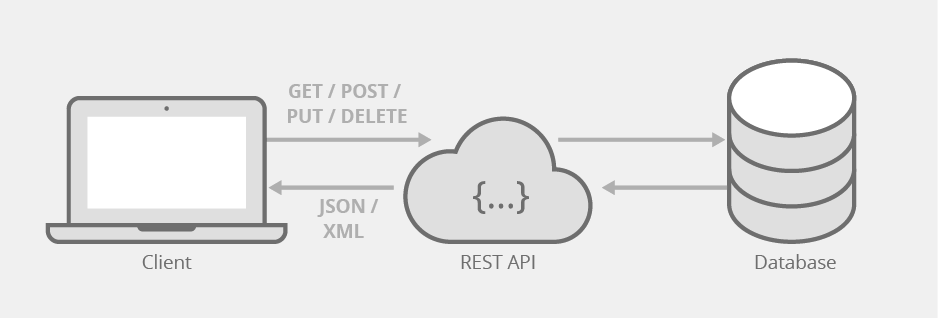
\includegraphics[width=0.9\textwidth]{./slike/app1}
\caption{REST arhitektura sustava [9]}
\label{fig:app1}
\end{figure}
%
REST \engl{Representational State Transfer} je arhitekturalni stil za oblikovanje servisa na webu. Kada klijent pošalje zahtjev za resursima prema REST poslužitelju, poslužitelj vraća trenutno stanje traženih resursa u bazi podataka [9]. \\

U razvijenoj aplikaciji, klijentsku stranu čini mobilni uređaj s pokrenutom klijentskom aplikacijom koja komunicira s poslužiteljskom stranom, tj. REST servisom. Klijent s REST servisom komunicira protokolom HTTP, koristeći zahtjeve GET i POST. HTTP je komunikacijski protokol koji omogućava dohvaćanje i slanje resursa na webu. Podaci se dohvaćaju GET zahtjevom, a šalju se koristeći POST zahtjev [20]. Podaci koji se šalju su u JSON formatu. JSON \engl{JavaScript Object Notation} je standardni format razmjene i pohrane podataka u obliku parova ključ-vrijednost \engl{key-value pairs} [21].\\

Poslužiteljsku stranu čini pokrenuti REST poslužitelj. Poslužitelj prima HTTP zahtjeve klijentske strane i na temelju traženih resursa formira zahtjeve prema bazi podataka. Poslužitelj s bazom podataka komunicira jezikom SQL. SQL \engl{Structured Query Language} je standardni jezik za komunikaciju i upravljanje relacijskim bazama podataka [22]. Temeljem povratne vrijednosti zahtjeva upućenih prema bazi podataka, poslužitelj klijentu vraća trenutno stanje traženih resursa.\\

Bazu podataka čini pokrenuti sustav za upravljanje bazom podataka \engl{DBMS-Database Management System} koji omogućava trajnu pohranu i pristup podacima u bazi. 
\newpage

\section{Korištene tehnologije i alati}
Aplikacija je izgrađena za operacijski sustav Android, uz korištenje programskog jezika Java i biblioteke Retrofit. Android je operacijski sustav otvorenog koda(eng. open source) temeljen na Linux jezgri \engl{Linux Kernel}, a koristi se u svim vrstama mobilnih uređaja, kao što su pametni telefoni i tableti [23]. Retrofit je HTTP klijentska biblioteka korištena za razvoj Java Android aplikacija koje komuniciraju s REST servisima na poslužiteljskoj strani [24]. Za potrebe razvoja poslužitelja korišten je razvojni okvir \engl{framework} Java Spring i biblioteke Spring Web, Spring Security, PostgreSQL Driver i Spring Data JPA. Spring je aplikacijski razvojni okvir za Java platformu, nudi mnoštvo biblioteka koje služe kao pomoć u ostvarivanju potrebnih funkcionalnosti aplikacija. Spring Web se koristi za izgradnju Spring REST servisa. Spring Security pomaže u implementaciji kontrole pristupa i autentifikacije za Spring servise. PostgreSQL Driver omogućava Spring aplikacijama povezivanje i uporabu PostgreSQL baze podataka. Spring Data JPA olakšava pristup i komunikaciju s bazom podataka koristeći Java kod [25]. Kao baza podataka korišten je PostgreSQL. To je sustav za upravljanje relacijskim bazama podataka \engl{rational database management system} otvorenog koda [26].\\
%
Programski alati korišteni za razvoj aplikacije su:
\begin{itemize}
\item[$\bullet$] Android Studio -- klijentska strana
\item[$\bullet$] Intellij IDEA -- serverska strana 
\item[$\bullet$] pgAdmin -- baza podataka
\item[$\bullet$] Visual Studio Code -- klasifikacija slika korištenjem modela duboke neuronske mreže
\end{itemize}

\section{Klijentska strana}
Klijentsku stranu sustava čini Android mobilna aplikacija. Aplikacija pruža intuitivno korisničko sučelje i ostvaruje korisnu primjenu razvijenog modela duboke neuronske mreže. U Android okruženju jedan "ekran" aplikacije je aktivnost \engl{Activity} i sastoji se od dva dijela: dizajna i funkcionalne logike. Dizajn i izgled korisničkog sučelja ostvaren je XML datotekama razmještaja, dok je za funkcionalnost sučelja zadužena pripadajuća datoteka s Java kodom. Razvijene aktivnosti s pripadajućim funkcionalnostima prikazane su u nastavku.\\

Prilikom pokretanja aplikacije otvara se aktivnost s početnim izbornikom. Kako je preduvjet za korištenje funkcionalnosti klasifikacije registracija i prijava u sustav, ovdje se korisniku nude opcije prelaska na te aktivnosti.
%
\begin{figure}[!h]
\centering
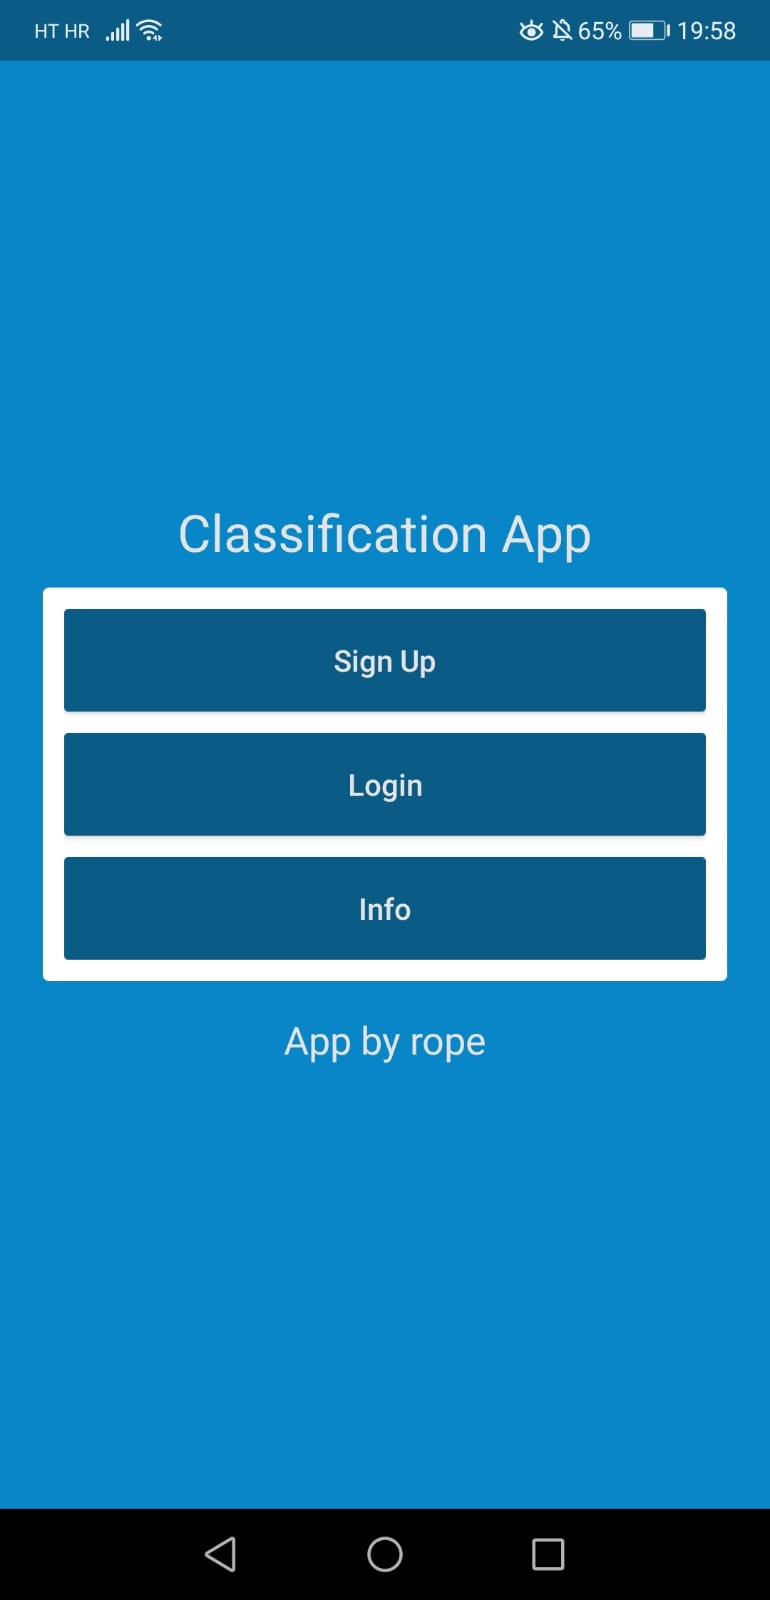
\includegraphics[width=0.32\textwidth]{./slike/app2}
\caption{Početni izbornik}
\label{fig:app2}
\minipage{0.32\textwidth}
  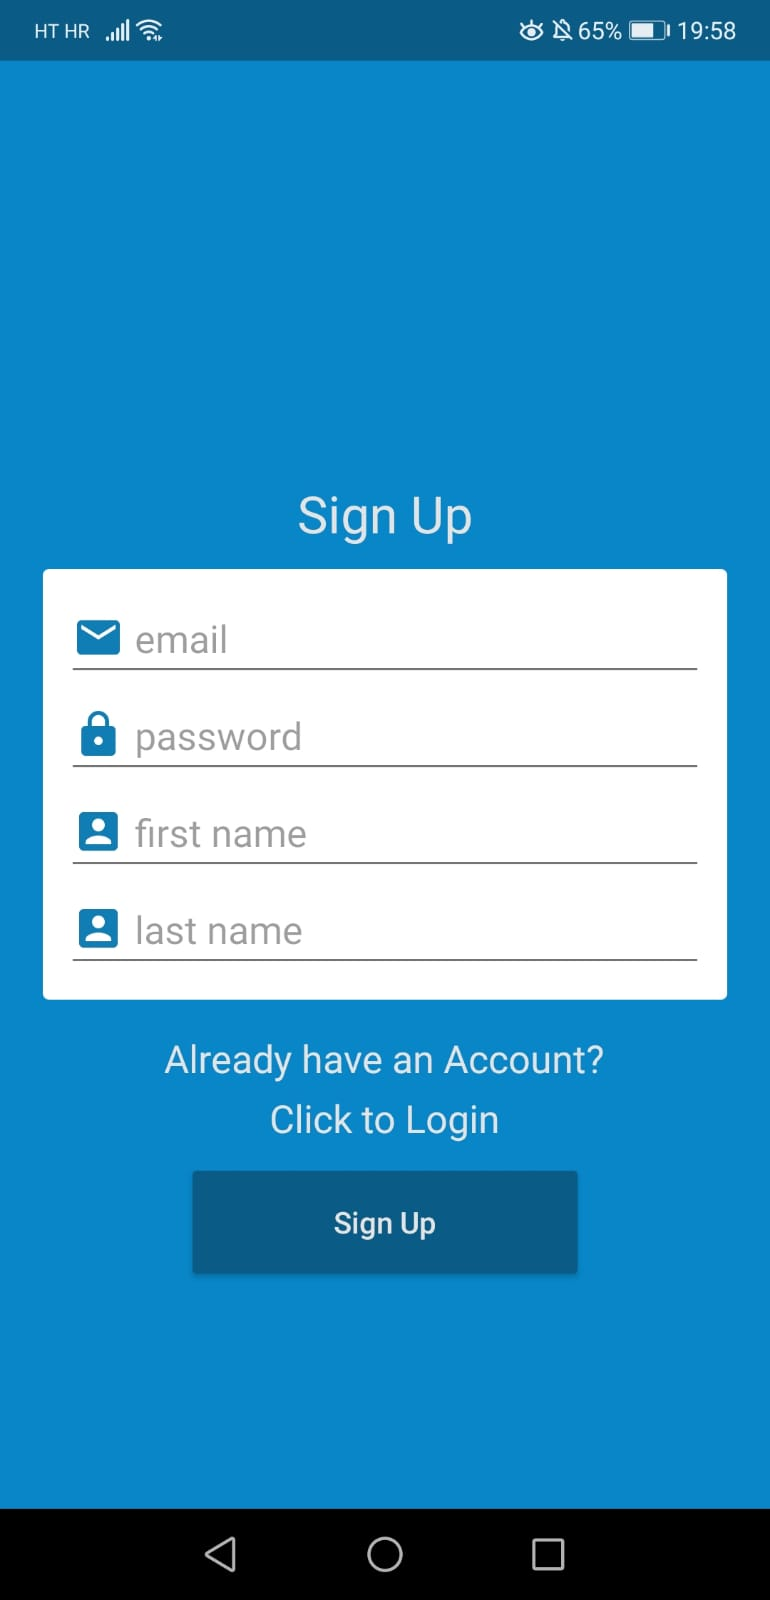
\includegraphics[width=1\textwidth]{./slike/app3}
	\caption{Registracija}
\label{fig:app2}
\endminipage\hfill
\minipage{0.32\textwidth}
  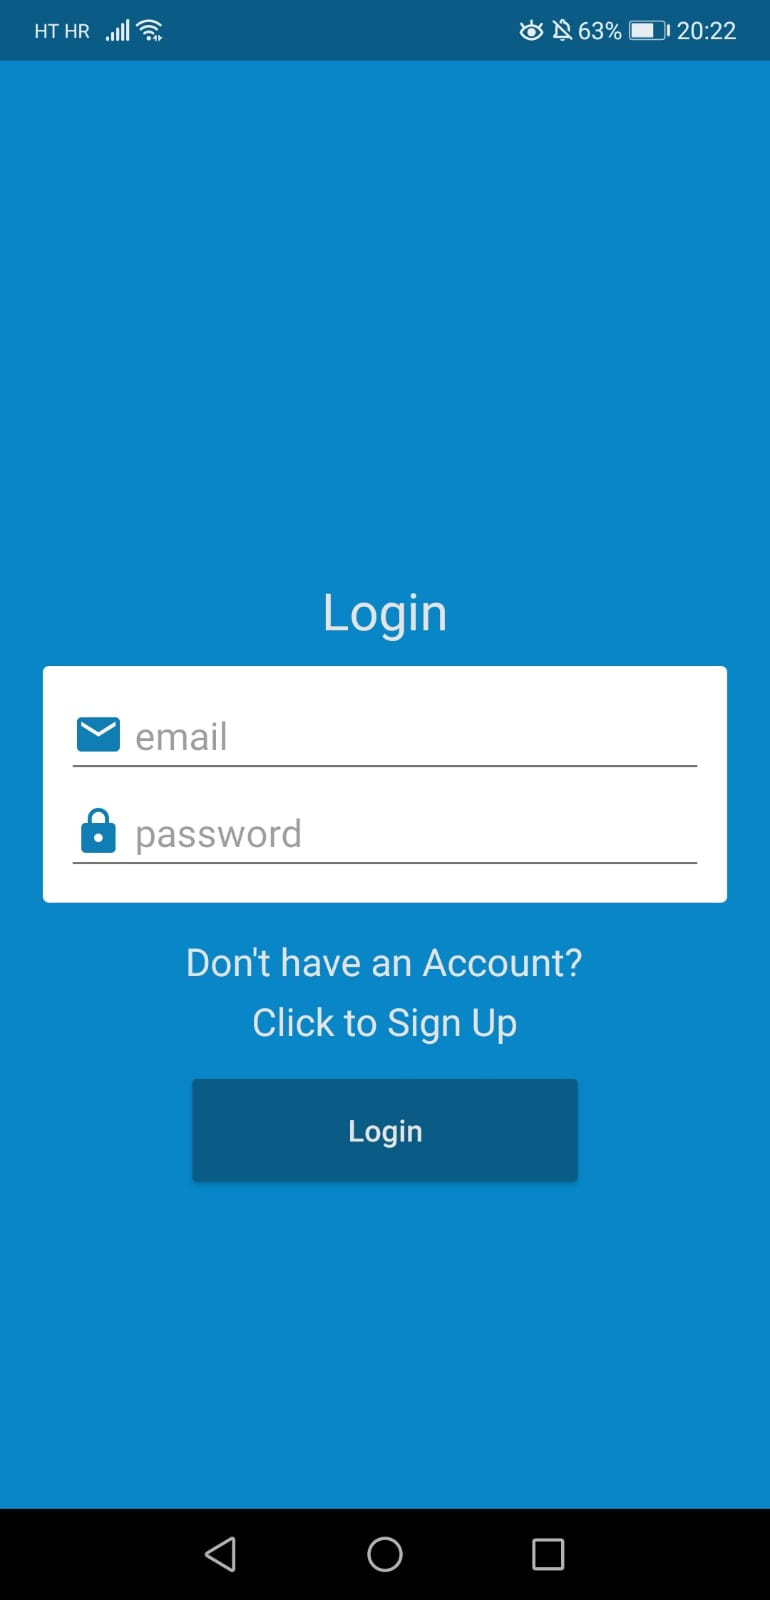
\includegraphics[width=1\textwidth]{./slike/app4}
	\caption{Login}
\label{fig:app2}
\endminipage\hfill
\minipage{0.32\textwidth}
  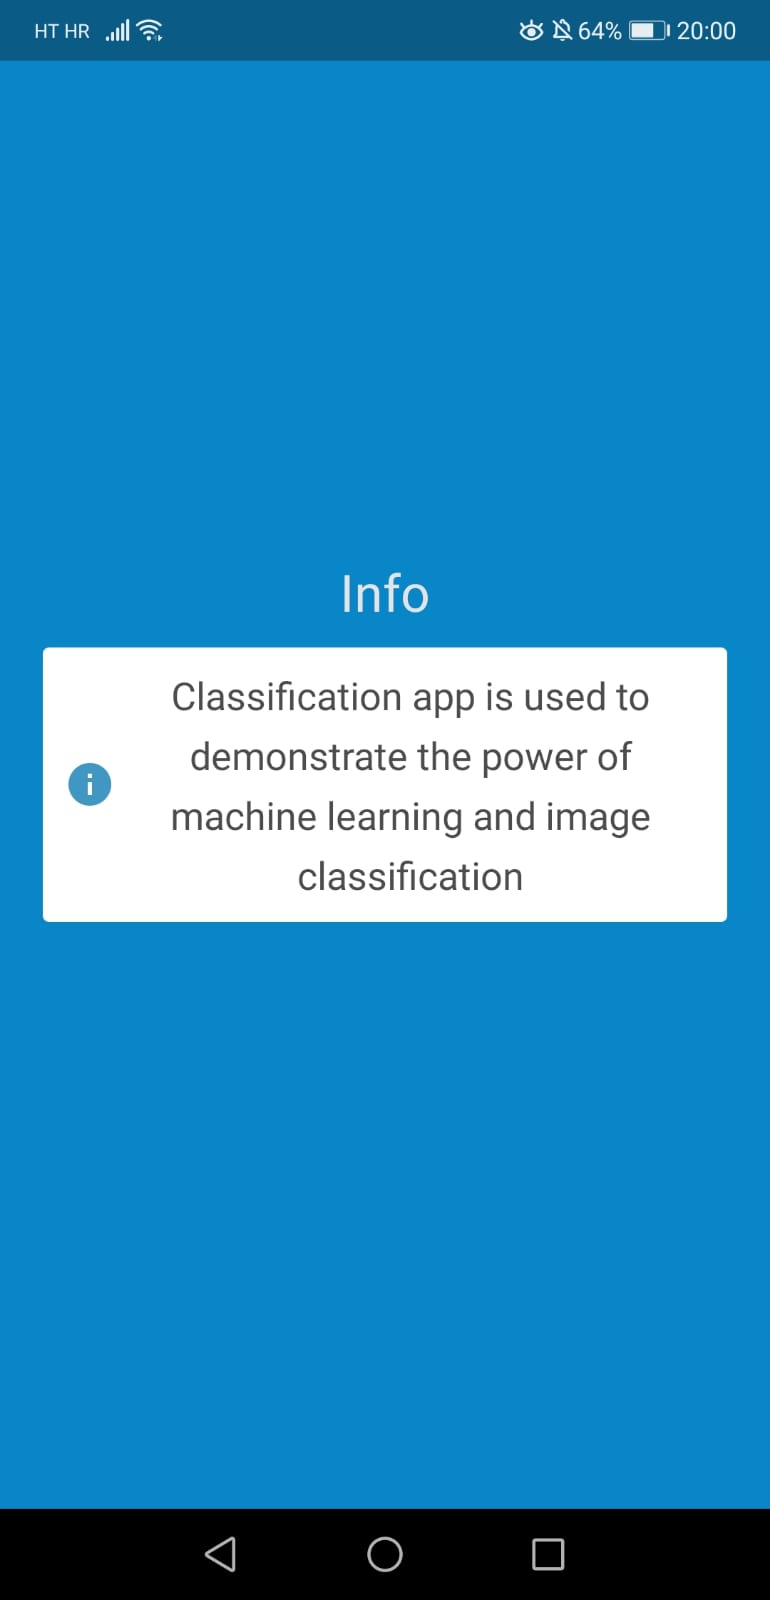
\includegraphics[width=1\textwidth]{./slike/app5}
	\caption{Info}
\label{fig:app2}
\endminipage\hfill
\end{figure}
%
\newpage
Za registraciju je u "Sign up" formu potrebno upisati email adresu, lozinku, ime i prezime. Klikom na gumb "Sign up" pokreće se validacija unesenih podataka. Provjerava se ispravan format email adrese i minimalna duljina lozinke, te postojanje unosa u poljima za ime i prezime. Nakon validacije uneseni podaci šalju se na poslužitelj korištenjem Retrofit POST zahtjeva. Ako neka od validacija ne prolazi podaci se ne šalju na poslužitelj i korisnika se upozorava na pogrešku.\\
%
\indent{}
Ako je registracija bila uspješna, moguće se logirati u sustav korištenjem forme za login, potrebno je upisati postojeći email i lozinku. Klikom na gumb "Login" pokreće se već spomenuta validacija za email i lozinku. Nakon validacije uneseni podaci šalju se na poslužitelj korištenjem Retrofit POST zahtjeva na koji poslužitelj odgovara statusom 200 OK u kojem uz osnovne korisničke podatke vraća kolačić za sjednicu \engl{session cookie}. Korisnički podaci koje poslužitelj vraća u odgovoru na login spremaju se u tzv. $Shared Preferences$ koji služi kao kontejner podataka za sve aktivnosti Android aplikacije, kako bi u svakoj mogli saznati podatak o trenutno logiranom korisniku.\\
%
\indent{}
Info aktivnost služi za informiranje korisnika o aplikaciji, a mogu joj pristupiti i neprijavljeni korisnici.\\
Nakon uspješnog logiranja u sustav uz skočnu poruku prikazuje se izbornik s opcijama prelaska na aktivnosti za klasifikaciju ("Classify"), pregled obavljenih klasifikacija ("Records") i odjavu iz sustava ("Logout").
%
\begin{figure}[!h]
\centering
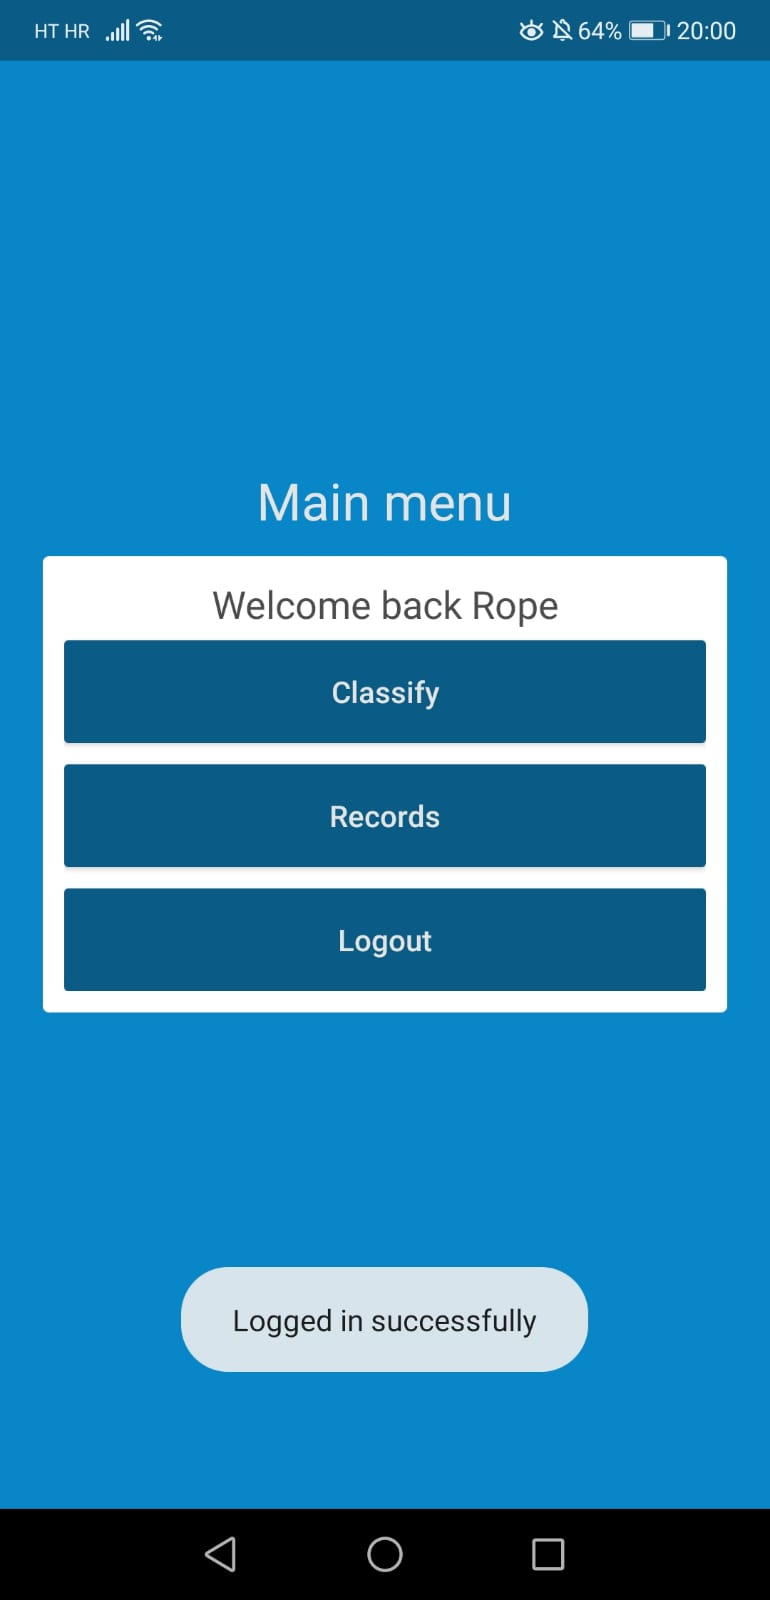
\includegraphics[width=0.3\textwidth]{./slike/app6}
\caption{Glavni izbornik}
\label{fig:app6}
\end{figure}
%
\newpage
%
\begin{figure}[!h]
\centering
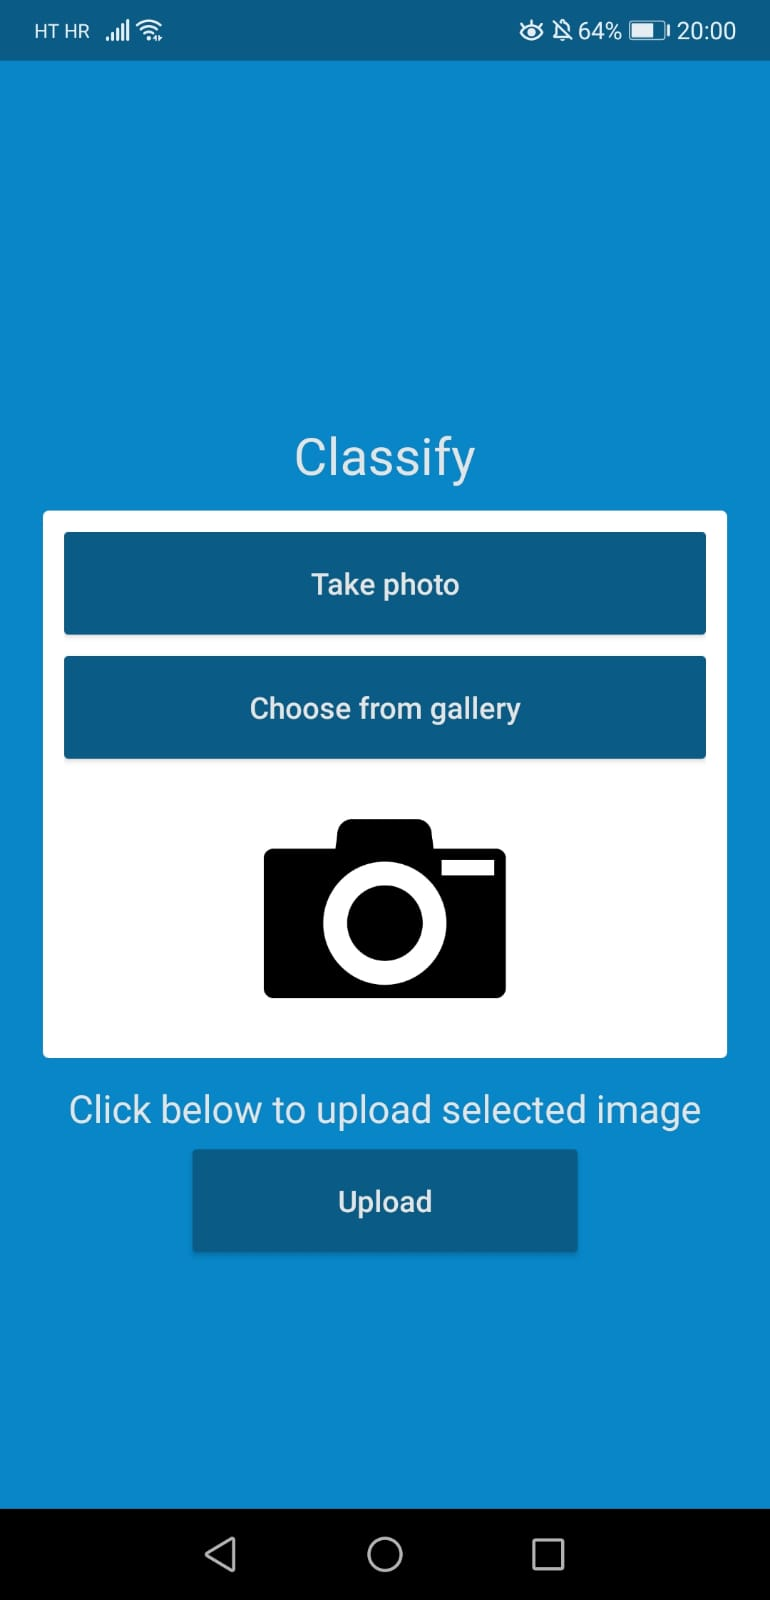
\includegraphics[width=0.32\textwidth]{./slike/app7}
\caption{Aktivnost za klasifikaciju}
\label{fig:app7}
\minipage{0.32\textwidth}
  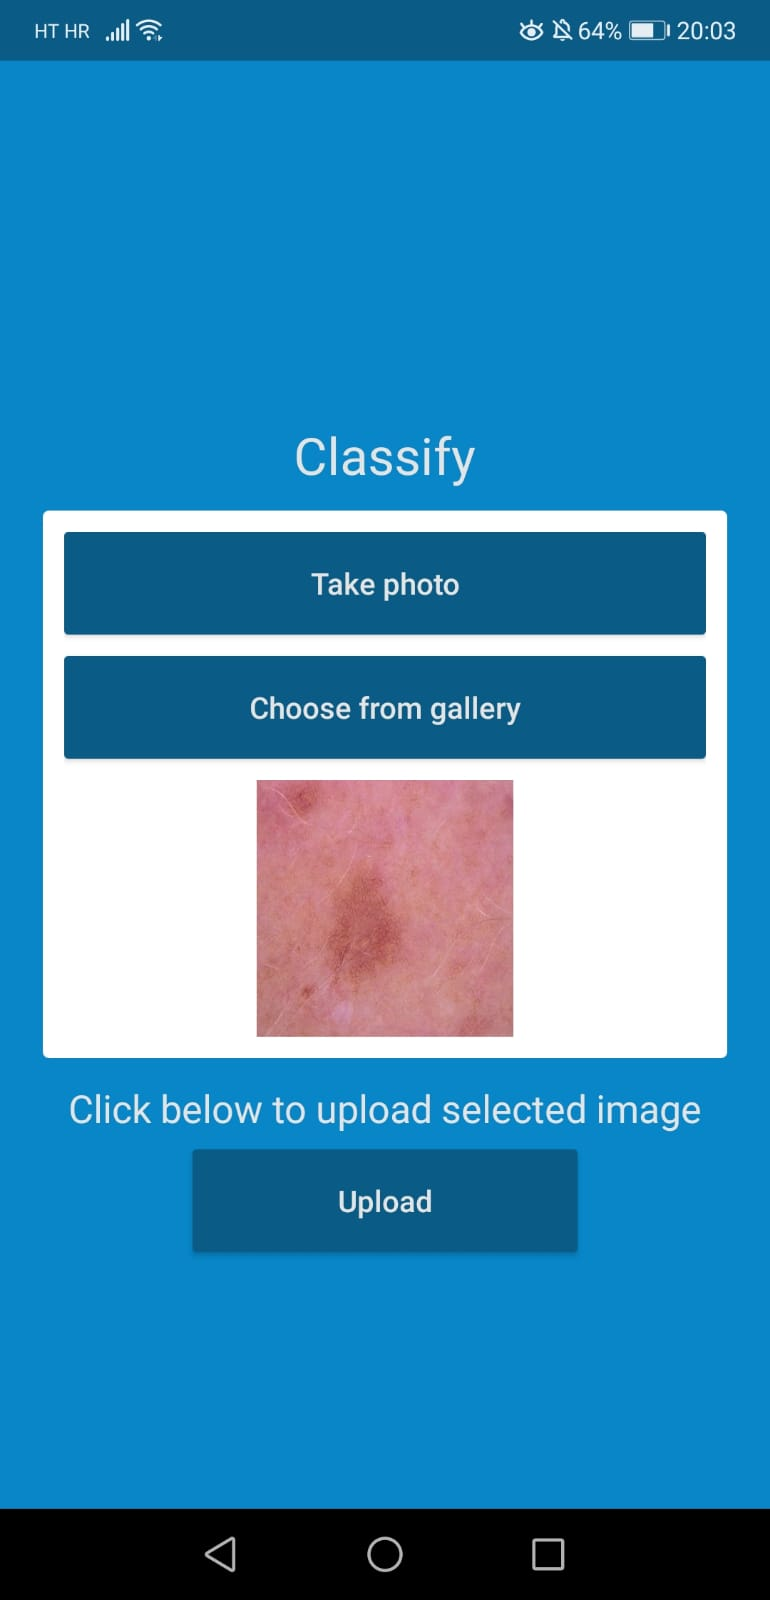
\includegraphics[width=1\textwidth]{./slike/app8}
	\caption{Odabir slike}
\label{fig:app8}
\endminipage\hfill
\minipage{0.32\textwidth}
  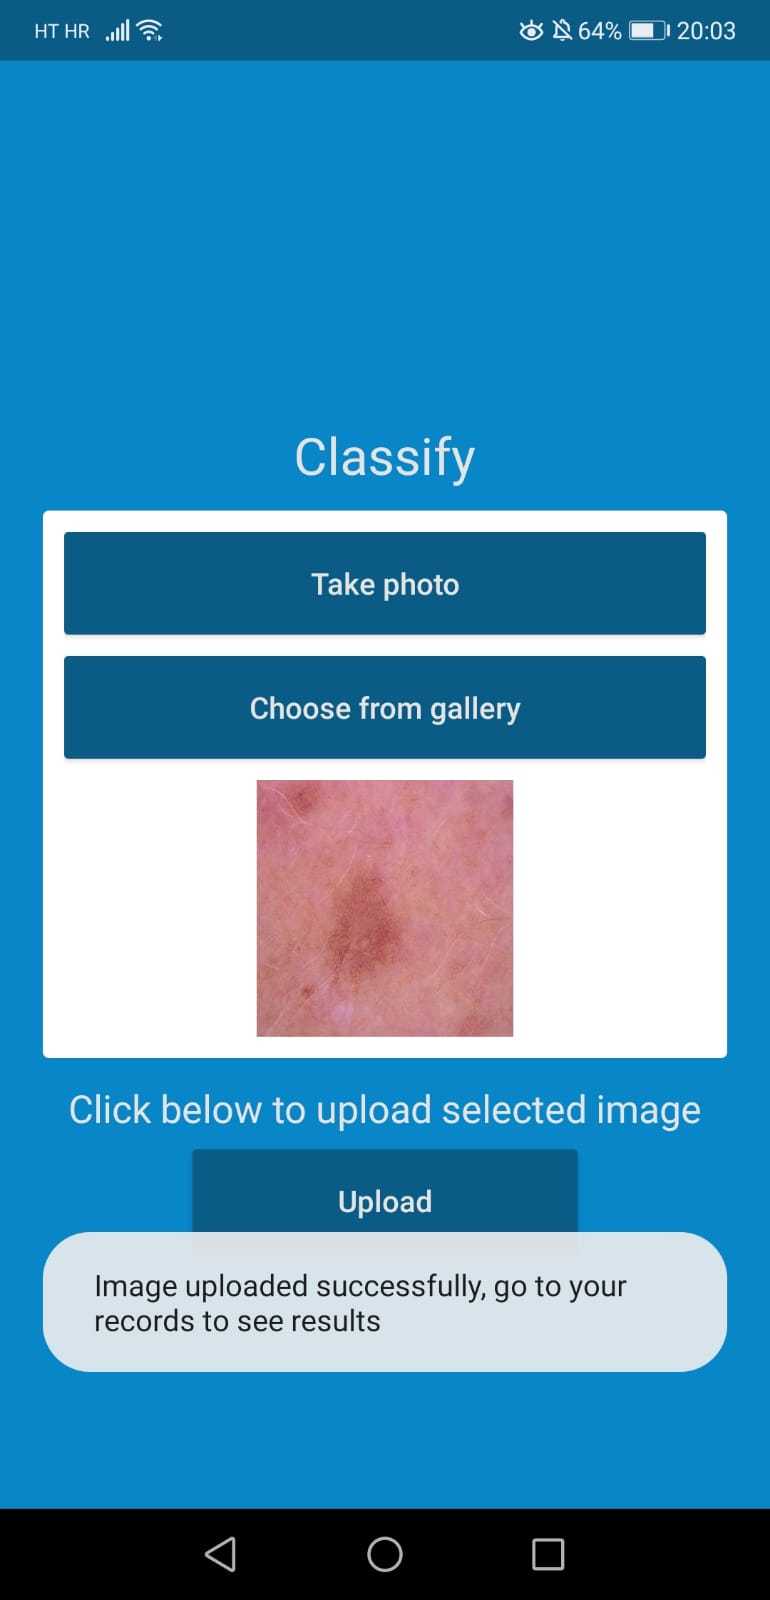
\includegraphics[width=1\textwidth]{./slike/app9}
	\caption{Skočna poruka}
\label{fig:app9}
\endminipage\hfill
\minipage{0.32\textwidth}
  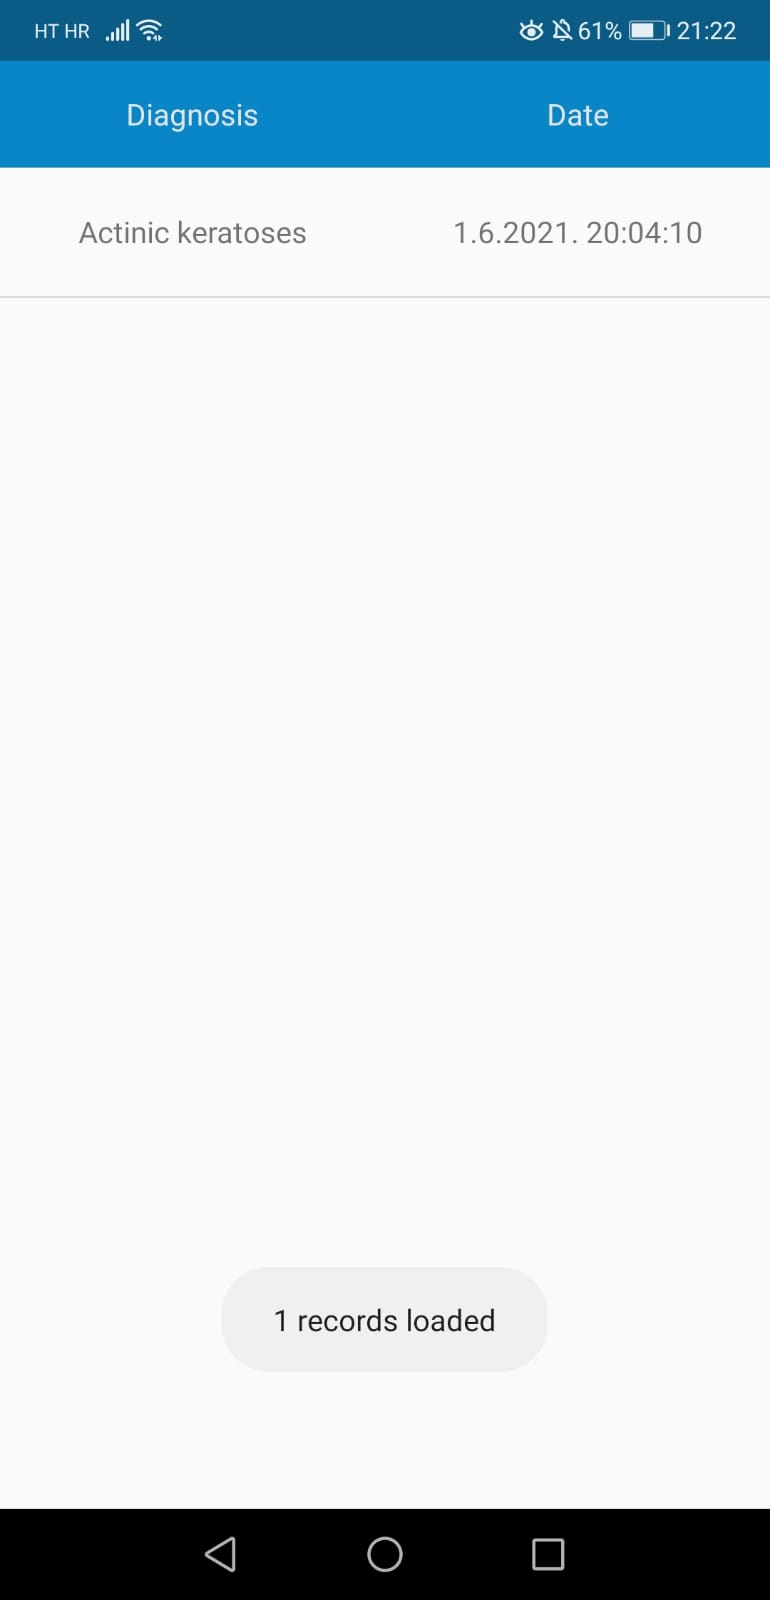
\includegraphics[width=1\textwidth]{./slike/app10}
	\caption{Rezultati}
\label{fig:app10}
\endminipage\hfill
\end{figure}
%
\newpage

Na slici 5.7 prikazana je aktivnost za klasifikaciju. U njoj je potrebno priložiti sliku koja će se slati poslužitelju. Aktivnost omogućava korištenje kamere za slikanje kožnog oboljenja ili odabir postojeće slike iz galerije. Ako se aplikacija koristi po prvi put, od korisnika će biti zatraženo dopuštenje za pristup kameri i galeriji pri odabiru tih aktivnosti. U slučaju da korisnik aplikaciji ne dopusti pristup tim resursima, aplikacija će se samo vratiti na prethodnu aktivnost. Nakon odabira slike ona se prikazuje umjetno $placeholder$ ikone fotoaparata i spremna je za slanje na poslužitelj, što je prikazano na slici 5.8. Konačno, klikom na gumb "Upload" odabrana slika šalje se na poslužitelj korištenjem Retrofit POST zahtjeva. Za vrijeme čekanja odgovora s poslužitelja korisniku se prikazuje $progress$ $bar$, a nakon uspješnog slanja i skočna poruka prikazana na slici 5.9. Također je osigurano da korisnik ne može slati zahtjev poslužitelju ako prethodno nije odabrao sliku, a ako dođe do greške prilikom klasifikacije na serveru, ispisuje se poruka o pogrešci ili timeouta u slučaju čekanja dužem od 10 sekundi.\\
%
\indent{}
Kako bi se prikazali rezultati klasifikacije potrebno je odabrati aktivnost "Records", prikazanu na slici 5.10. U toj aktivnosti prikazan je popis svih obavljenih klasifikacija uz odgovarajuće dijagnoze kožnih oboljenja i vrijeme slanja slike na poslužitelj.

\section{Poslužiteljska strana}
Poslužiteljsku stranu sustava čini Spring REST poslužitelj. Taj poslužitelj prima klijentske HTTP zahtjeve na temelju kojih obavlja upite prema bazi podataka i kao povratnu vrijednost klijenti u HTTP odgovoru vraća trenutno stanje traženih resursa [9].\\
%
\indent{}
Spring REST poslužitelji izgrađeni su u troslojnoj arhitekturi \engl{three tier architecture}. Ta arhitektura raspoređuje odgovornosti u aplikaciji na tri dijela: prezentacijski sloj \engl{presentation layer}, servisni sloj \engl{business layer} i podatkovni sloj \engl{data access layer}.\\
%
\indent{}
U prezentacijskom sloju nalaze se REST kontroleri koji prihvaćaju HTTP zahtjeve na određenim putanjama, uz deserijalizaciju podataka poslanih u JSON formatu. Dodatno, s obzirom na korištenje biblioteke Spring Security, uz svaki zahtjev na zaštićenu putanju potrebno je poslati podatke za autentifikaciju. Ako je autentifikacija uspjela nastavlja se obrada zahtjeva, a u suprotnom se klijentu vraća statusni kod "401 Unauthorized" i prekida se daljnja obrada zahtjeva. Prihvaćeni zahtjev se, ovisno o putanji na koju je poslan, prosljeđuje servisnom sloju na obradu.\\
%
\indent{}
Na servisnom sloju nalazi se kod koji odgovara poslovnoj logici sustava, ovdje se još jednom obavlja validacija podataka nalik onoj na klijentskoj strani. Servisni sloj ima pristup podatkovnom sloju, koji služi kao veza između aplikacije i baze podataka. Nakon obrade proslijeđenog HTTP zahtjeva, servisni sloj ga prosljeđuje podatkovnom sloju.\\
%
\indent{}
U podatkovnom sloju se proslijeđeni zahtjev prevodi u SQL upit prema bazi podataka korištenjem biblioteke Spring Data JPA. Kada baza podataka vrati izlazni status s odgovorom, on se prosljeđuje od podatkovnog sloja natrag preko servisnog i prezentacijskog sloja pa sve do klijenta.
%
\begin{figure}[!h]
\centering
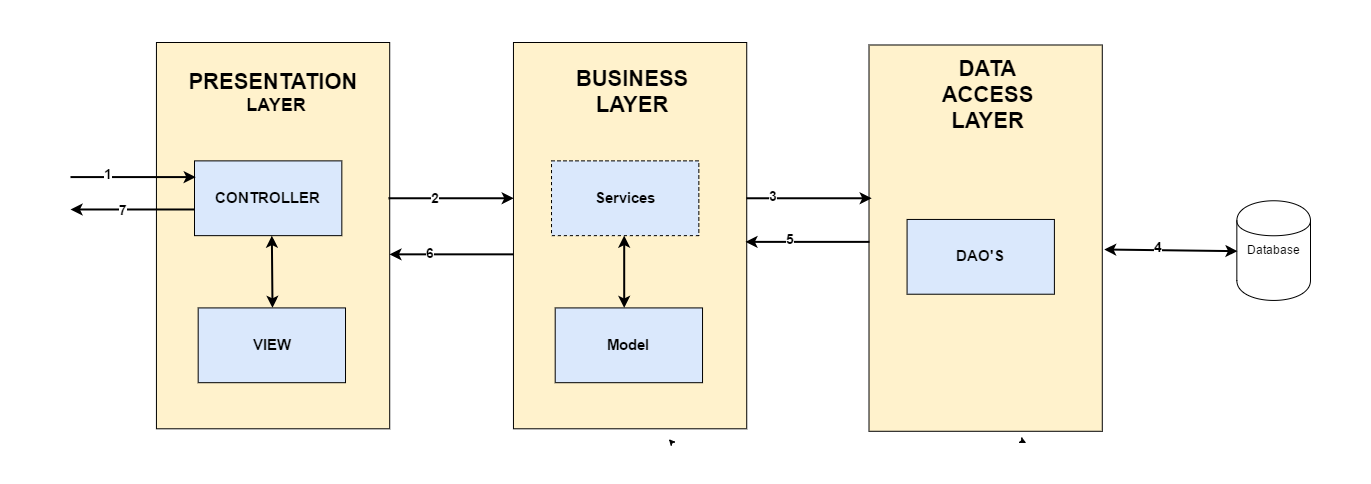
\includegraphics[width=1\textwidth]{./slike/springArch}
\caption{Troslojna arhitektura [10]}
\label{fig:springArch}
\end{figure}
%
\\
Na razvijenom REST poslužitelju bitno je naglasiti sljedeće dijelove troslojne arhitekture, uz kratak opis funkcionalnosti.\\
%
Prezentacijski sloj:
\begin{itemize}
\item[$\bullet$] RegisterController -- prihvat zahtjeva za registraciju
\item[$\bullet$] LoginController -- prihvat zahtjeva za login
\item[$\bullet$] RecordController -- prihvat zahtjeva sa slikama za klasifikaciju
\end{itemize}
%
Servisni sloj:
\begin{itemize}
\item[$\bullet$] PatientServiceJpa -- logika za stvaranje i traženje korisnika u bazi podataka
\item[$\bullet$] RecordServiceJpa -- logika za stvaranje i traženje klasifikacija slika kožnih oboljenja u bazi podataka, ovdje se pokreće skripta s Python kodom u kojem se razvijenim modelom duboke neuronske mreže obavlja klasifikacije poslane slike
\end{itemize}
%
Podatkovni sloj:
\begin{itemize}
\item[$\bullet$] PatientRepository -- pristup podacima o korisnicima
\item[$\bullet$] RecordRepository -- pristup podacima o obavljenim klasifikacijama
\end{itemize}

\section{Baza podataka}
Dio zadužen za bazu podataka u razvijenom sustavu čini postgreSQL, koji osim pohrane pruža i rukovanje podacima u relacijskoj bazi podataka. Bazi pristupamo preko podatkovnog sloja poslužiteljske strane sustava. Dijagram tablica u bazi podataka s pripadajućim tipovima podataka po pojedinim stupcima dani su u nastavku.\\
%
\begin{figure}[!h]
\centering
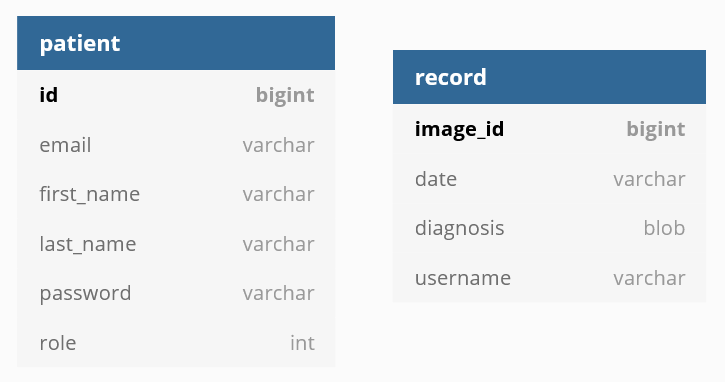
\includegraphics[width=0.9\textwidth]{./slike/dijagram}
\caption{Dijagram baze podataka}
\label{fig:dijagram}
\end{figure}
%
\\
U tablici "patient" spremljeni su podaci o korisnicima, a podaci o klasifikacijama njihovih kožnih lezija nalaze se u tablici "record". Važno je napomenuti da su tipovi podataka po stupcima točno definirani i provjeravaju se prilikom obrade SQL upita nad bazom podataka. Tako se i u ovom dijelu sustava obavlja validacija podataka, uz spomenute validacije na klijentskoj i poslužiteljskoj strani. Ako dođe do neslaganja između očekivanih i poslanih tipova podataka baza javlja grešku i zaustavlja daljnje izvođenje upita.


\chapter{Zaključak}
Razvijeni model duboke neuronske mreže sa zadovoljavajućom točnošću klasificira kožne lezije na temelju slika kože, a mobilna aplikacija koja ga koristi ispunjava postavljene funkcionalne zahtjeve. Aplikacija je osmišljena kao demonstracija praktične primjene modela dubokog učenja. Unaprijeđena verzija ove aplikacije koja bi mogla s većom točnošću klasificirati više od 7 klasa kožnih oboljenja imala bi potencijal za praktičnu uporabu. Takva aplikacija mogla bi se razvijati u smjeru pomoćnog alata u dermatološkoj dijagnostici, no nikako kao zamjena za medicinske stručnjake.\\
%
\indent{}
Radom na izradi ovakvog sustava stečena su iskustva u izgradnji Keras modela dubokog učenja, razvoja aplikacija za operacijski sustav Android i implementaciji Spring REST poslužitelja. 


%\bibliography{literatura}
%\bibliographystyle{fer}

\chapter{literatura}

\noindent{}[1] Daniel Hand, The Relationship between Artificial Intelligence (AI), Machine Learning (ML) \& Deep Learning (DL), 15.4.2020., \url{https://www.linkedin.com/pulse/relationship-between-artificial-intelligence-ai-machine-daniel-hand?articleId=6656073786821050368}, 20.5.2021.\\

\noindent{}[2] Porcelain Signapore, 5 Fun Facts About Skin, 3.11.2011., \url{https://porcelainskin.com/prologue/5-fun-facts-about-your-skin/}, 20.5.2021.\\

\noindent{}[3] Artem Oppermann, What is Deep Learning and How does it work?, 12.11.2019., \url{https://towardsdatascience.com/what-is-deep-learning-and-how-does-it-work-2ce44bb692ac}, 20.5.2021.\\

\noindent{}[4] Gavril Ognjanovski, Everything you need to know about Neural Networks and Backpropagation — Machine Learning Easy and Fun, 14.1.2019., \url{https://towardsdatascience.com/everything-you-need-to-know-about-neural-networks-and-backpropagation-machine-learning-made-easy-e5285bc2be3a}, 20.5.2021.\\

\noindent{}[5] Buduma, N. Fundamentals of Deep Learning: Convolutional Neural Networks. 1. izdanje. SAD: O'Reilly, 2017.\\

\noindent{}[6] Anirban Ray, 2016., Quora, \url{https://www.quora.com/What-is-meant-by-feature-maps-in-convolutional-neural-networks}, 21.5.2021.\\

\noindent{}[7] Sumit Saha, A Comprehensive Guide to Convolutional Neural Networks — the ELI5 way, 15.12.2018., \url{https://towardsdatascience.com/a-comprehensive-guide-to-convolutional-neural-networks-the-eli5-way-3bd2b1164a53}, 24.5.2021.\\\\

\noindent{}[8] Juliana Negrini de Araujo, HAM10000: Analysis and Model Comparison, 3.1.2021., \url{https://www.kaggle.com/jnegrini/ham10000-analysis-and-model-comparison}, 28.5.2021.\\

\noindent{}[9] Aveek Das, Create REST APIs in Python using Flask, 12.3.2021., \url{https://www.sqlshack.com/create-rest-apis-in-python-using-flask/}, 29.5.2021.\\

\noindent{}[10] Stack Overflow, Spring MVC and Three Tier Architecture, \url{https://stackoverflow.com/questions/44096677/spring-mvc-and-three-tier-architecture}, 29.5.2021.\\

\noindent{}[11] Chris Nicholson, Artificial Intelligence (AI) vs. Machine Learning vs. Deep Learning, \url{https://wiki.pathmind.com/ai-vs-machine-learning-vs-deep-learning}, 20.5.2021.\\

\noindent{}[12] Marina Chatterjee, Top 20 Applications of Deep Learning in 2021 Across Industries, 19.2.2019., \url{https://www.mygreatlearning.com/blog/deep-learning-applications/}, 20.5.2021.\\

\noindent{}[13] Markus Schmitt, Artificial Intelligence in Medicine, \url{https://www.datarevenue.com/en-blog/artificial-intelligence-in-medicine}, 20.5.2021.\\

\noindent{}[14] Šitum, M. Dermatovenerologija. 1. izdanje. Zagreb: Medicinska naklada, 2018.\\

\noindent{}[15] Harvard Dataverse, The HAM10000 dataset, a large collection of multi-source dermatoscopic images of common pigmented skin lesions, \url{https://dataverse.harvard.edu/dataset.xhtml?persistentId=doi:10.7910/DVN/DBW86T}, 22.5.2021.\\

\noindent{}[16] Arc, Convolutional Neural Network, 25.12.2018., \url{https://towardsdatascience.com/convolutional-neural-network-17fb77e76c05}, 25.5.2021.\\

\noindent{}[17] Keras, \url{https://keras.io/}\\

\noindent{}[18] NumPy, \url{https://numpy.org/}\\

\noindent{}[19] Pandas, \url{https://pandas.pydata.org/}\\

\noindent{}[20] HTTP Overview, \url{https://developer.mozilla.org/en-US/docs/Web/HTTP/Overview}\\

\noindent{}[21] JSON - introduction, \url{https://www.w3schools.com/js/js_json_intro.asp}\\

\noindent{}[22] Introduction to SQL, \url{https://www.w3schools.com/sql/sql_intro.asp}\\

\noindent{}[23] Android, \url{https://www.android.com/}\\

\noindent{}[24] Retrofit, \url{https://square.github.io/retrofit/}\\

\noindent{}[25] Spring, \url{https://spring.io/}\\

\noindent{}[26] PostgreSQL, \url{https://www.postgresql.org/}\\





\begin{sazetak}
Ovim radom demonstrirana je praktična primjena modela dubokog učenja. Prikazan je način izgradnje modela za klasifikaciju kožnih oboljenja iz slika kože i mobilne aplikacije koja ga koristi. 

\kljucnerijeci{Duboko učenje, duboke neuronske mreže, Keras, klasifikacija, Android, Spring, postgreSQL, kožna oboljenja, mobilna aplikacija}
\end{sazetak}


% TODO: Navedite naslov na engleskom jeziku.
\engtitle{Mobile application for the classification of skin diseases from skin images }
\begin{abstract}
This paper demonstrates the practical application of the deep learning model. The method of building a model for the classification of skin diseases from skin images and the mobile application that uses it is presented. 

\keywords{Deep learning, deep neural networks, Keras, classification, Android, Spring, postgreSQL, skin diseases, mobile application}
\end{abstract}

\end{document}
